%!TEX root = ../dokumentation.tex

\chapter{Abstract Prototype 1}

%Seite 1
\begin{figure}[H]
\centering
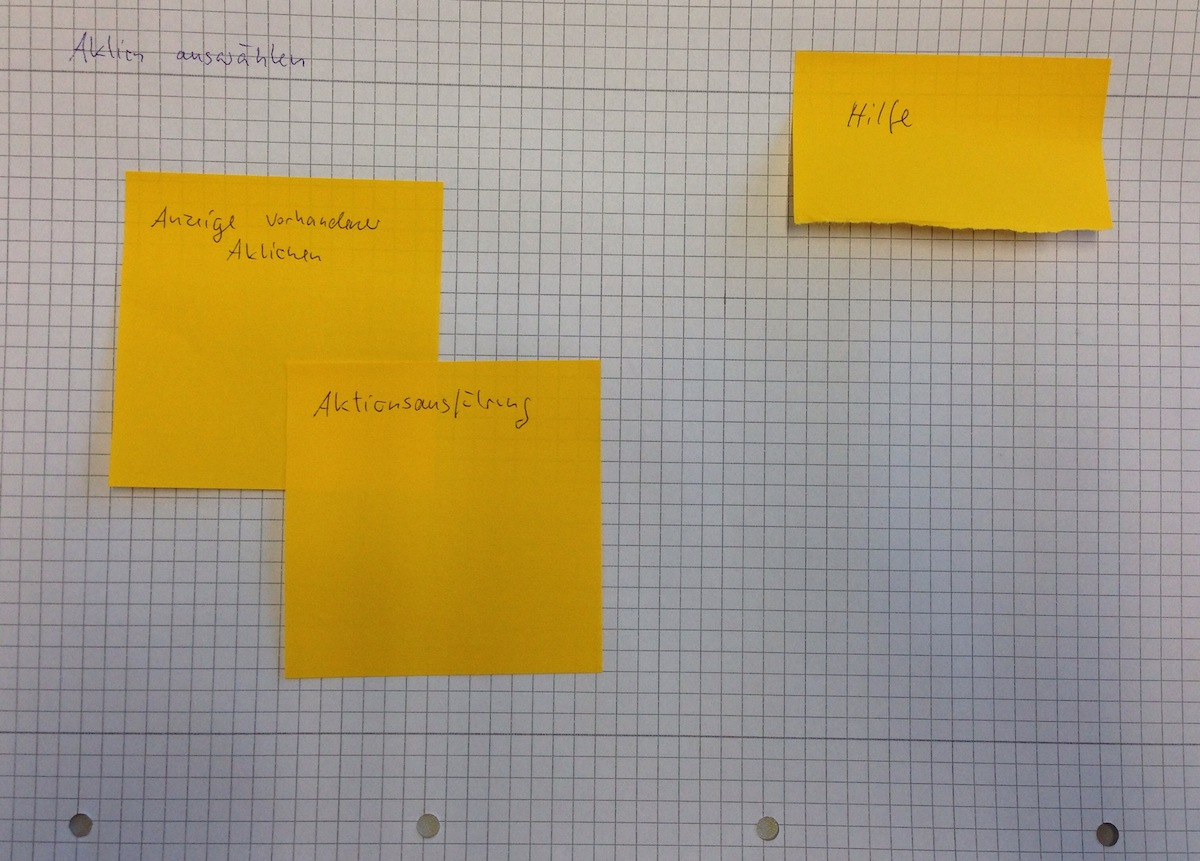
\includegraphics[width=0.85\textwidth]{./images/abstract/version1/aktionAuswaehlen.JPG}
\caption{Interaction Context AP1: aktionAuswählen}
\label{interfaceContents20}
\end{figure}

\begin{figure}[H]
\centering
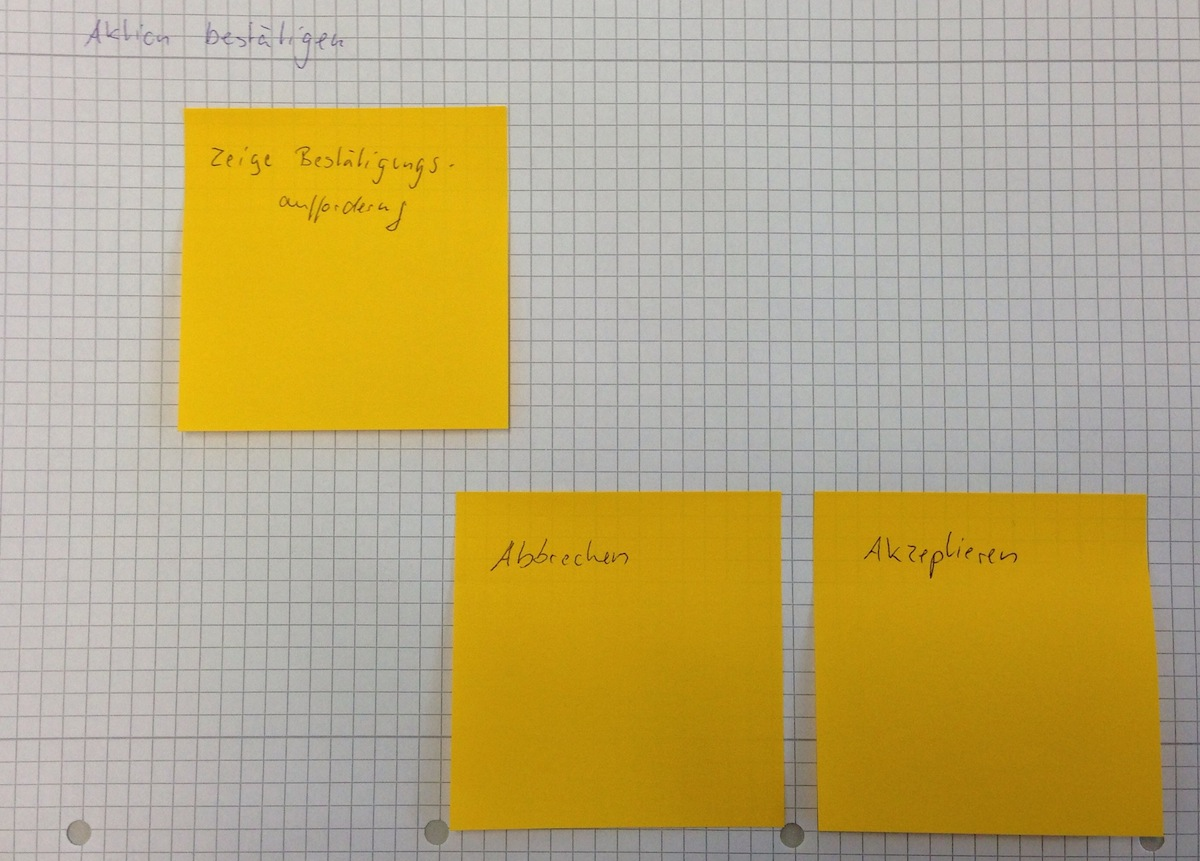
\includegraphics[width=0.85\textwidth]{./images/abstract/version1/aktionBestaetigen.JPG}
\caption{Interaction Context AP1: aktionBestätigen}
\label{interfaceContents21}
\end{figure}


%Seite 2
\begin{figure}[H]
\centering
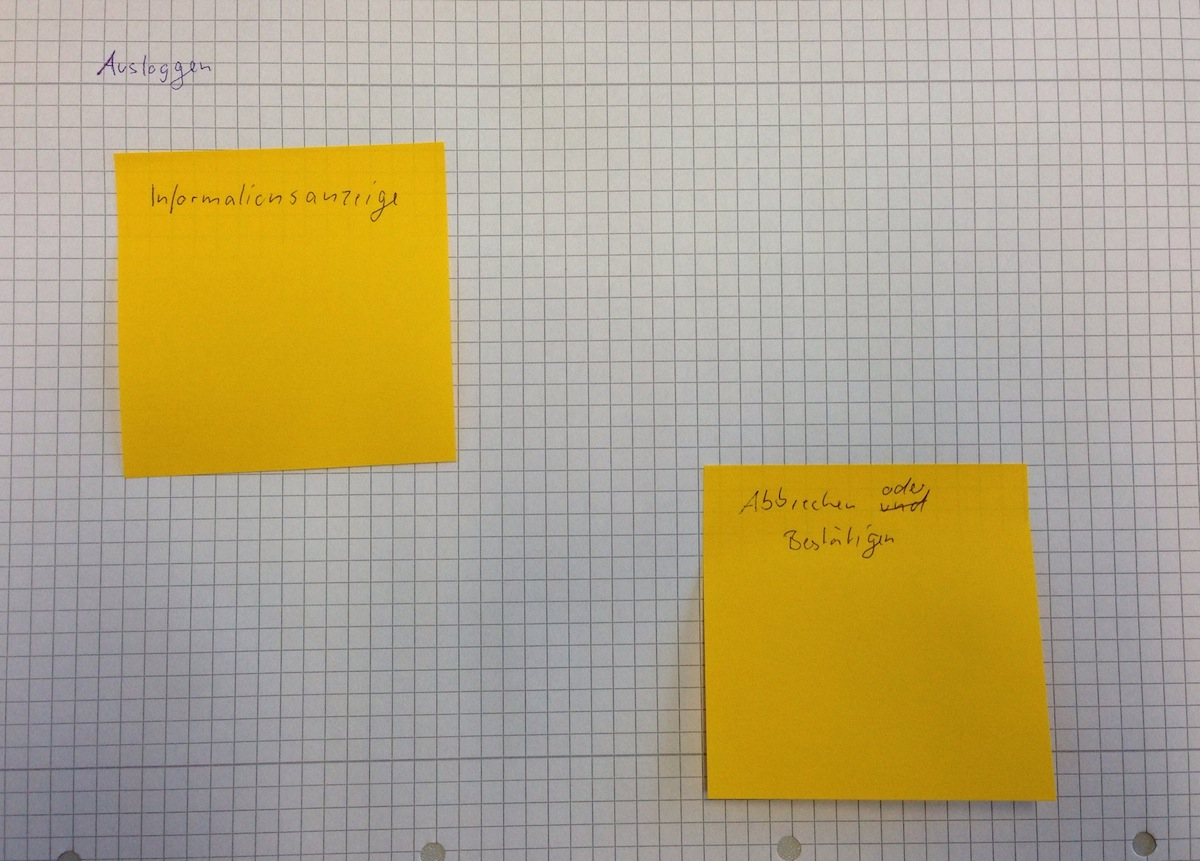
\includegraphics[width=0.85\textwidth]{./images/abstract/version1/ausloggen.JPG}
\caption{Interaction Context AP1: ausloggen}
\label{interfaceContents22}
\end{figure}

\begin{figure}[H]
\centering
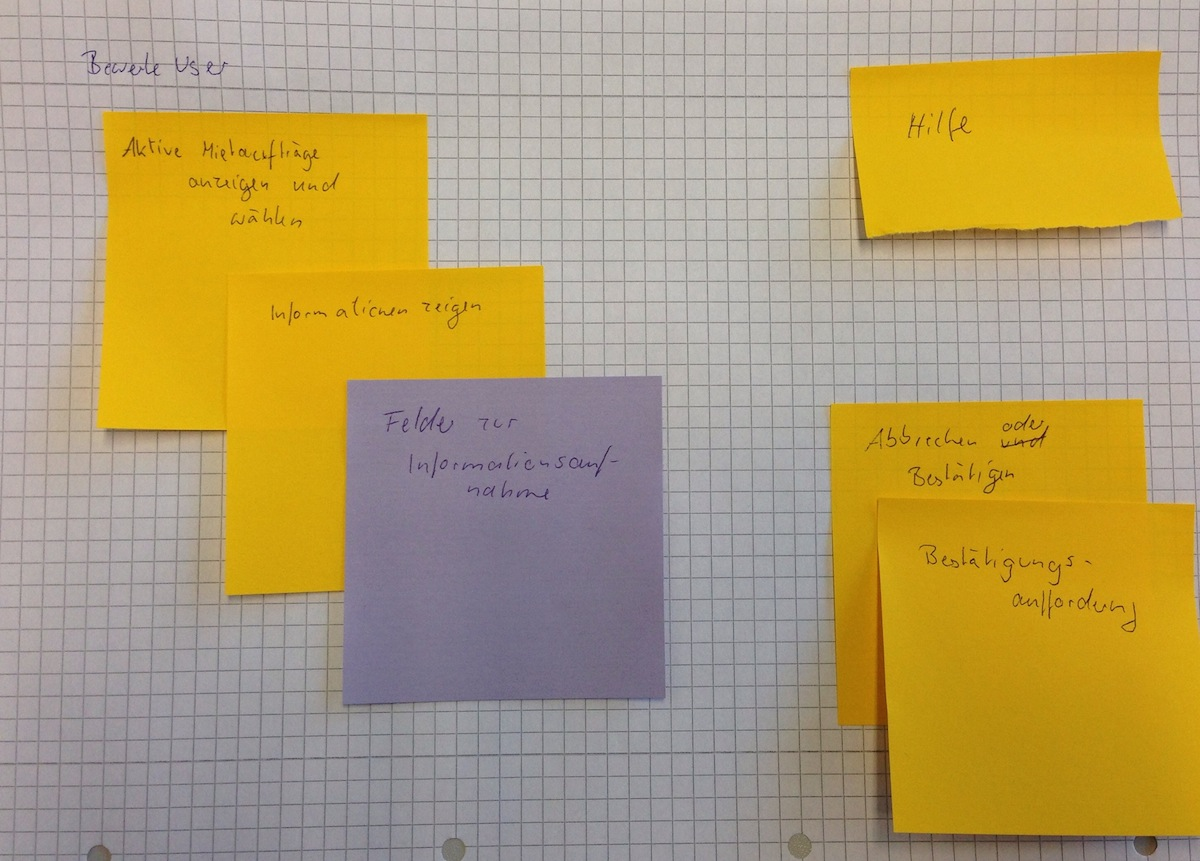
\includegraphics[width=0.85\textwidth]{./images/abstract/version1/bewerteUser.JPG}
\caption{Interaction Context AP1: bewerteUser}
\label{interfaceContents23}
\end{figure}


%Seite 3
\begin{figure}[H]
\centering
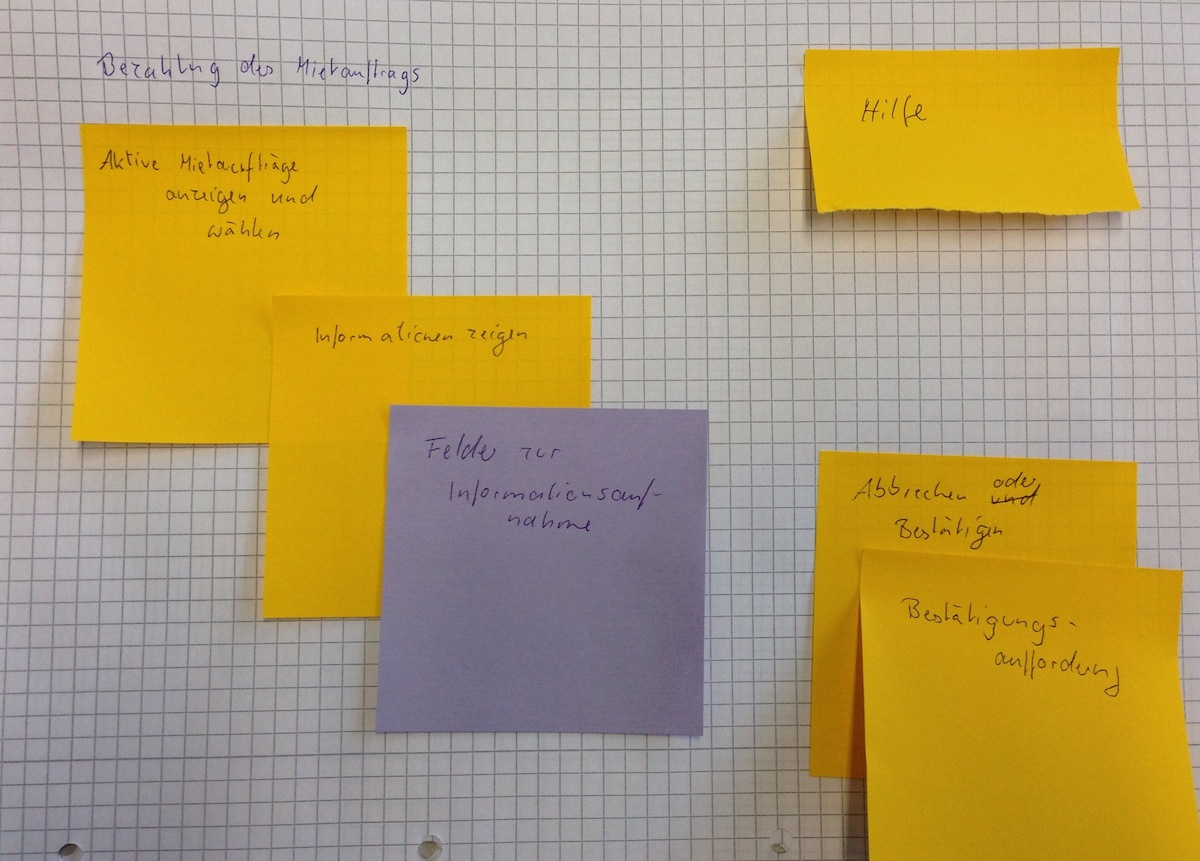
\includegraphics[width=0.85\textwidth]{./images/abstract/version1/bezahlungDesMietauftrags.JPG}
\caption{Interaction Context AP1: bezahlungDesMietauftrags}
\label{interfaceContents24}
\end{figure}

\begin{figure}[H]
\centering
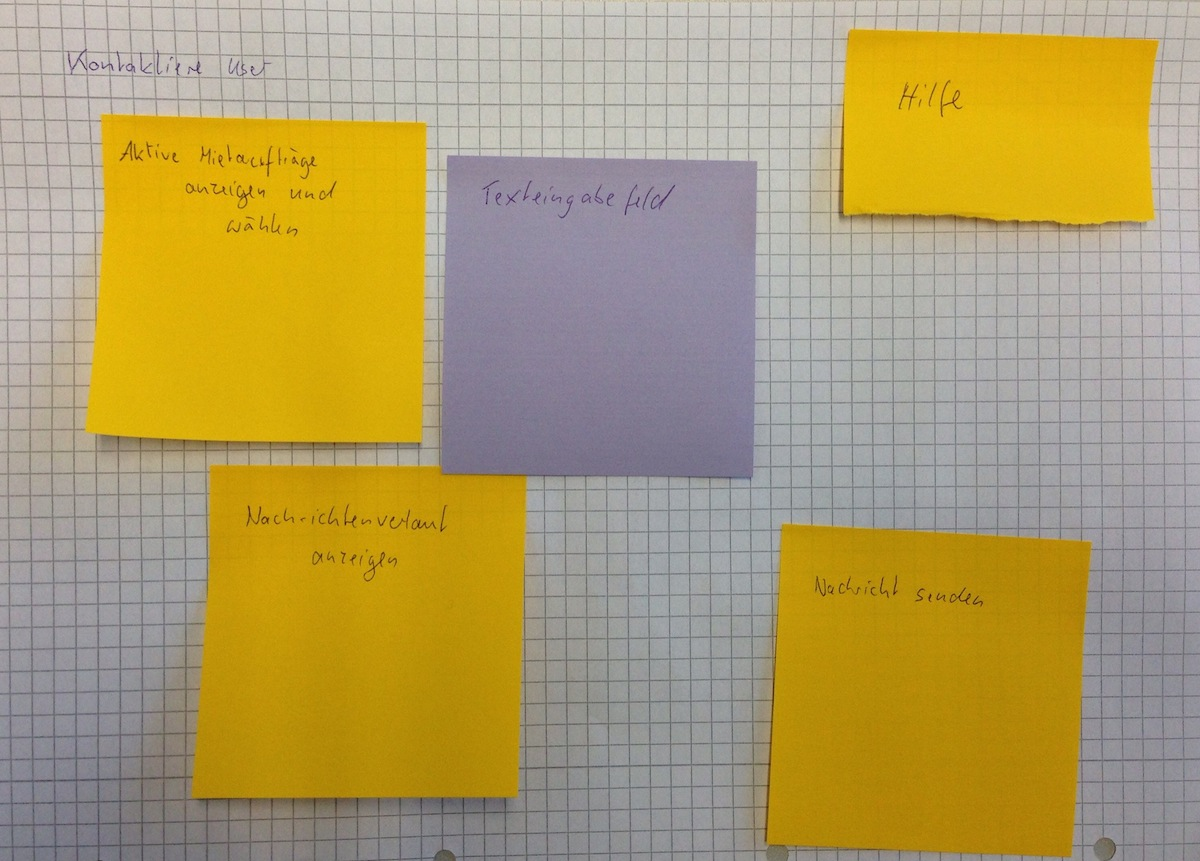
\includegraphics[width=0.85\textwidth]{./images/abstract/version1/kontaktiereUser.JPG}
\caption{Interaction Context AP1: kontaktiereUser}
\label{interfaceContents25}
\end{figure}


%Seite 4
\begin{figure}[H]
\centering
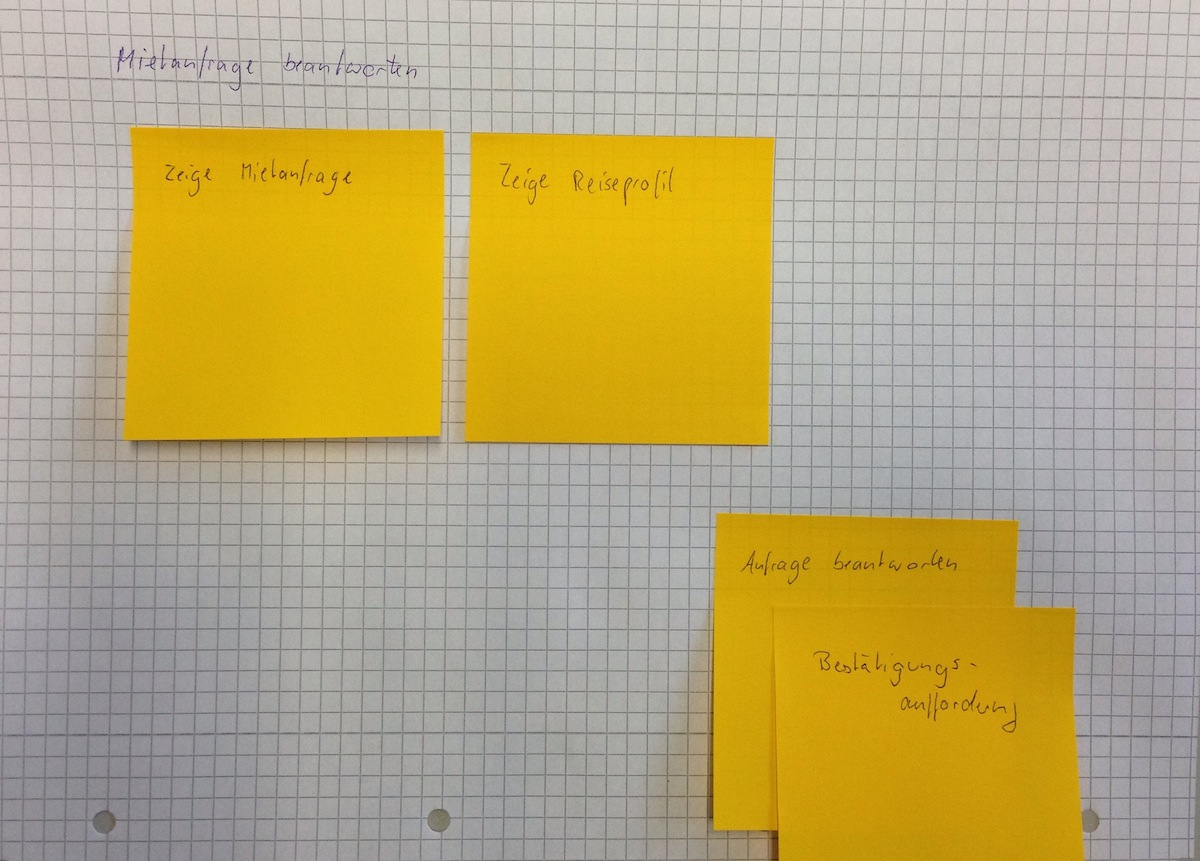
\includegraphics[width=0.85\textwidth]{./images/abstract/version1/mietanfrageBeantworten.JPG}
\caption{Interaction Context AP1: mietanfrageBeantworten}
\label{interfaceContents26}
\end{figure}

\begin{figure}[H]
\centering
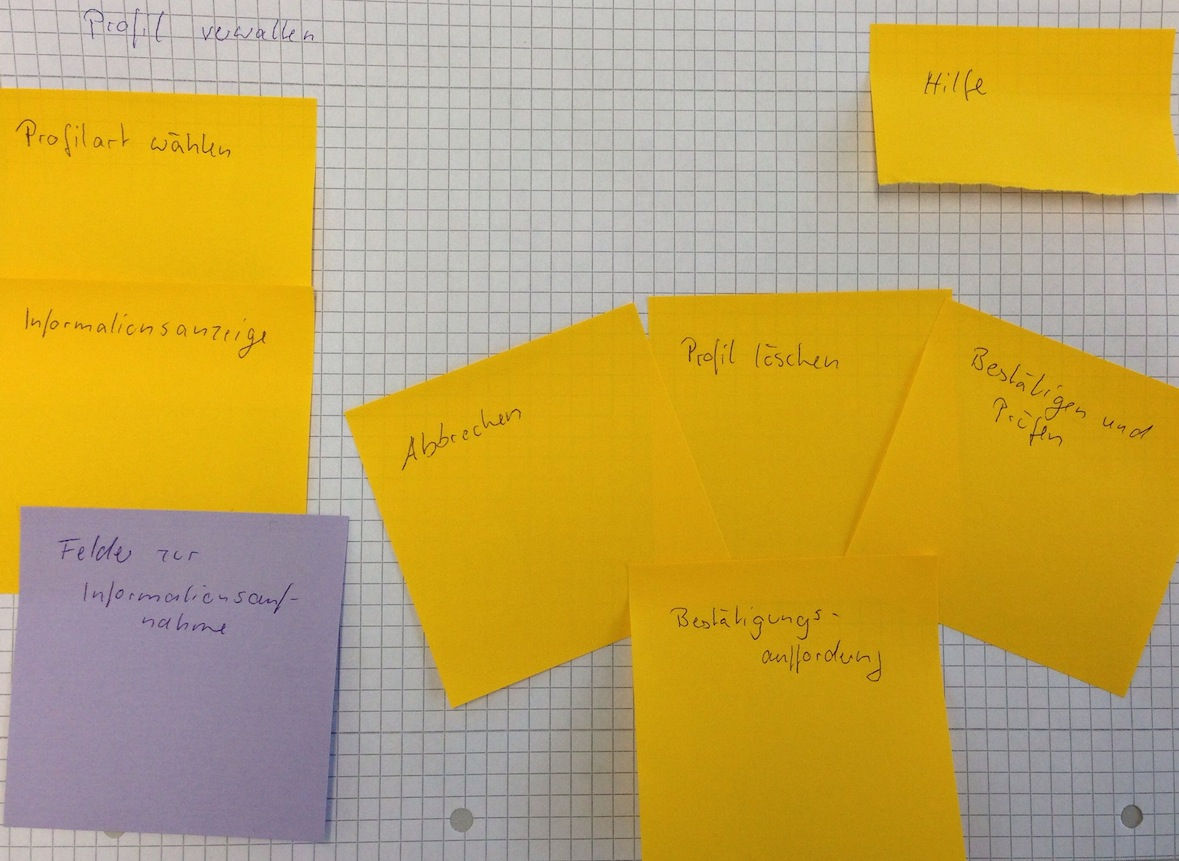
\includegraphics[width=0.85\textwidth]{./images/abstract/version1/profilVerwalten.JPG}
\caption{Interaction Context AP1: profilVerwalten}
\label{interfaceContents27}
\end{figure}


%Seite 5
\begin{figure}[H]
\centering
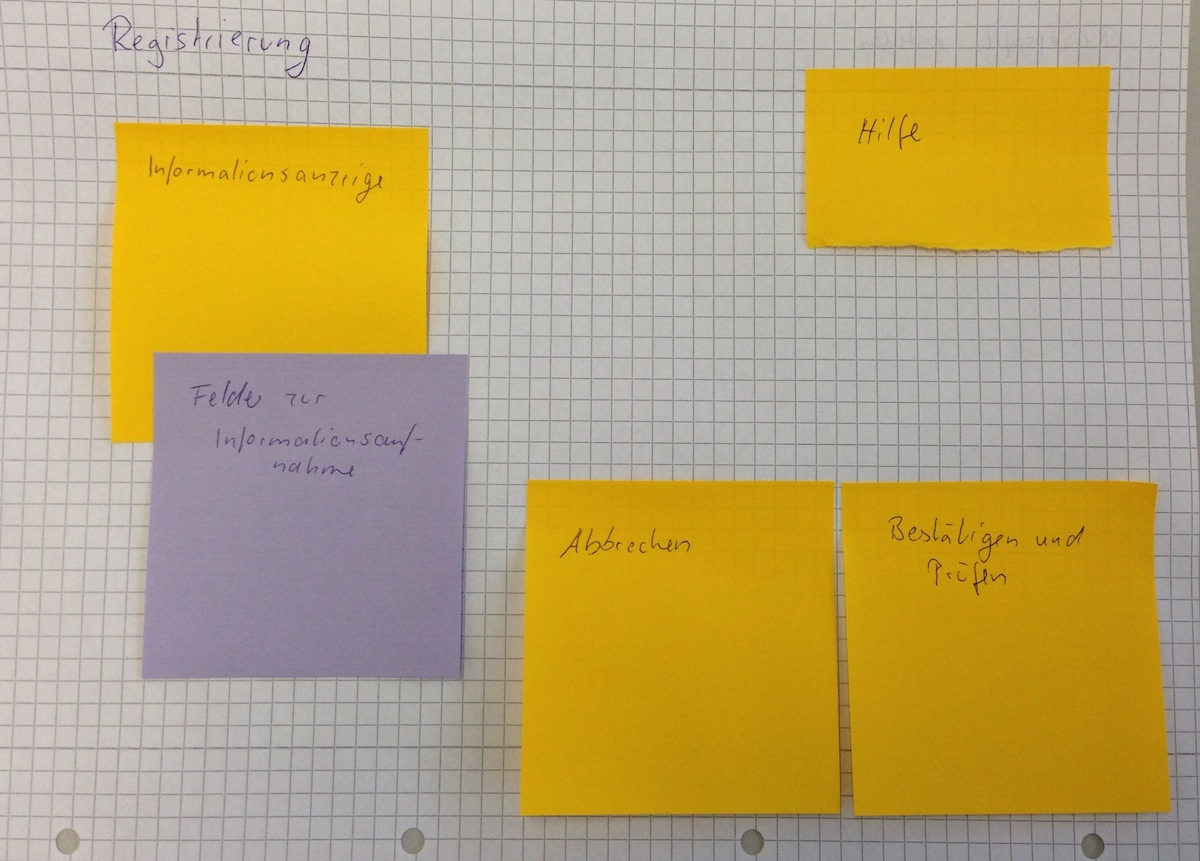
\includegraphics[width=0.85\textwidth]{./images/abstract/version1/registrierung.JPG}
\caption{Interaction Context AP1: registrierung}
\label{interfaceContents28}
\end{figure}

\begin{figure}[H]
\centering
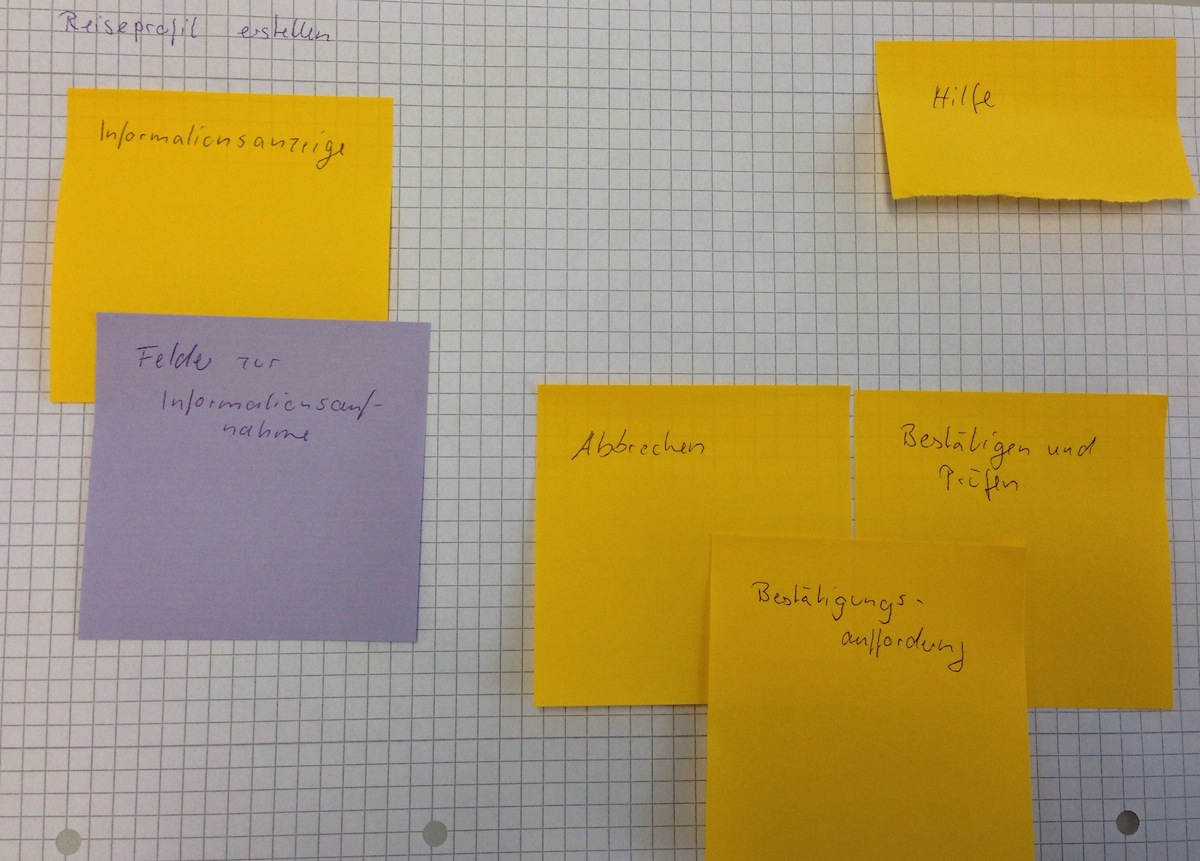
\includegraphics[width=0.85\textwidth]{./images/abstract/version1/reiseprofilErstellen.JPG}
\caption{Interaction Context AP1: reiseprofilErstellen}
\label{interfaceContents29}
\end{figure}

%Seite 6
\begin{figure}[H]
\centering
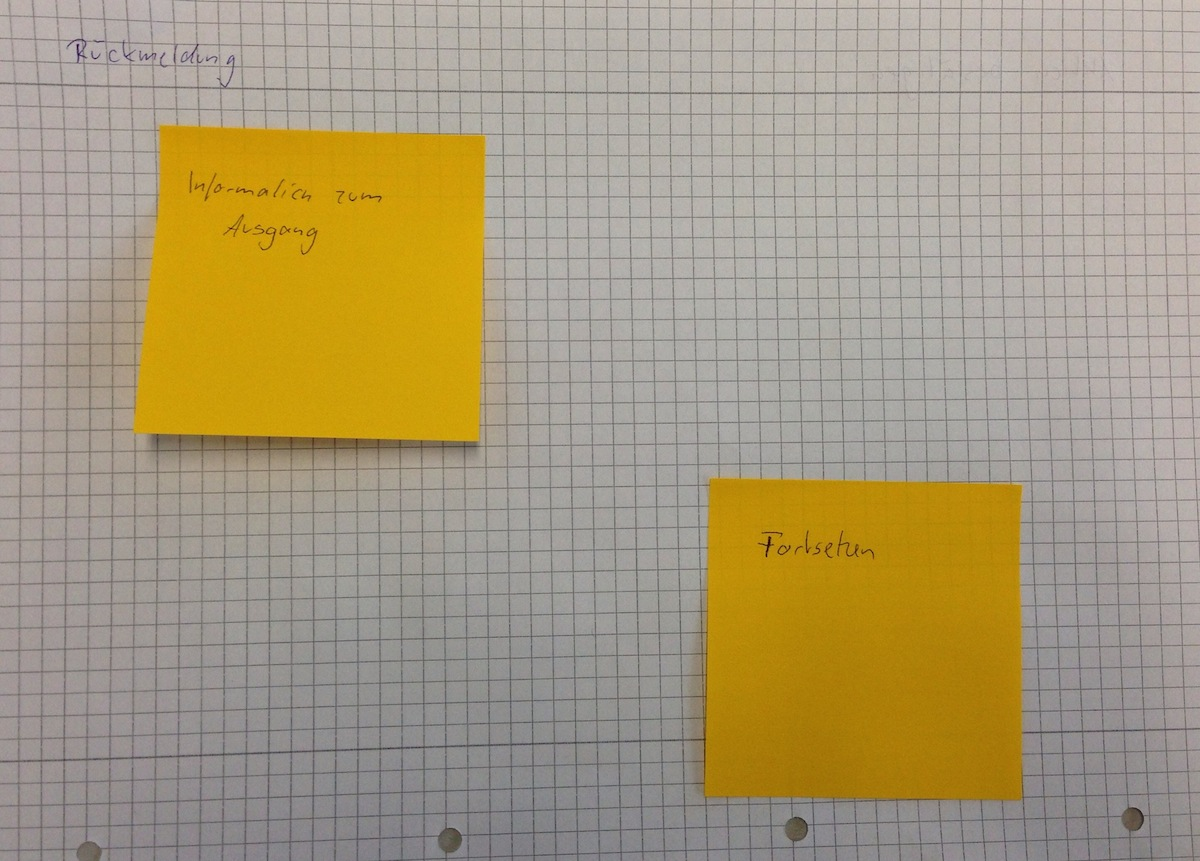
\includegraphics[width=0.85\textwidth]{./images/abstract/version1/rueckmeldung.JPG}
\caption{Interaction Context AP1: rueckmeldung}
\label{interfaceContents30}
\end{figure}

\begin{figure}[H]
\centering
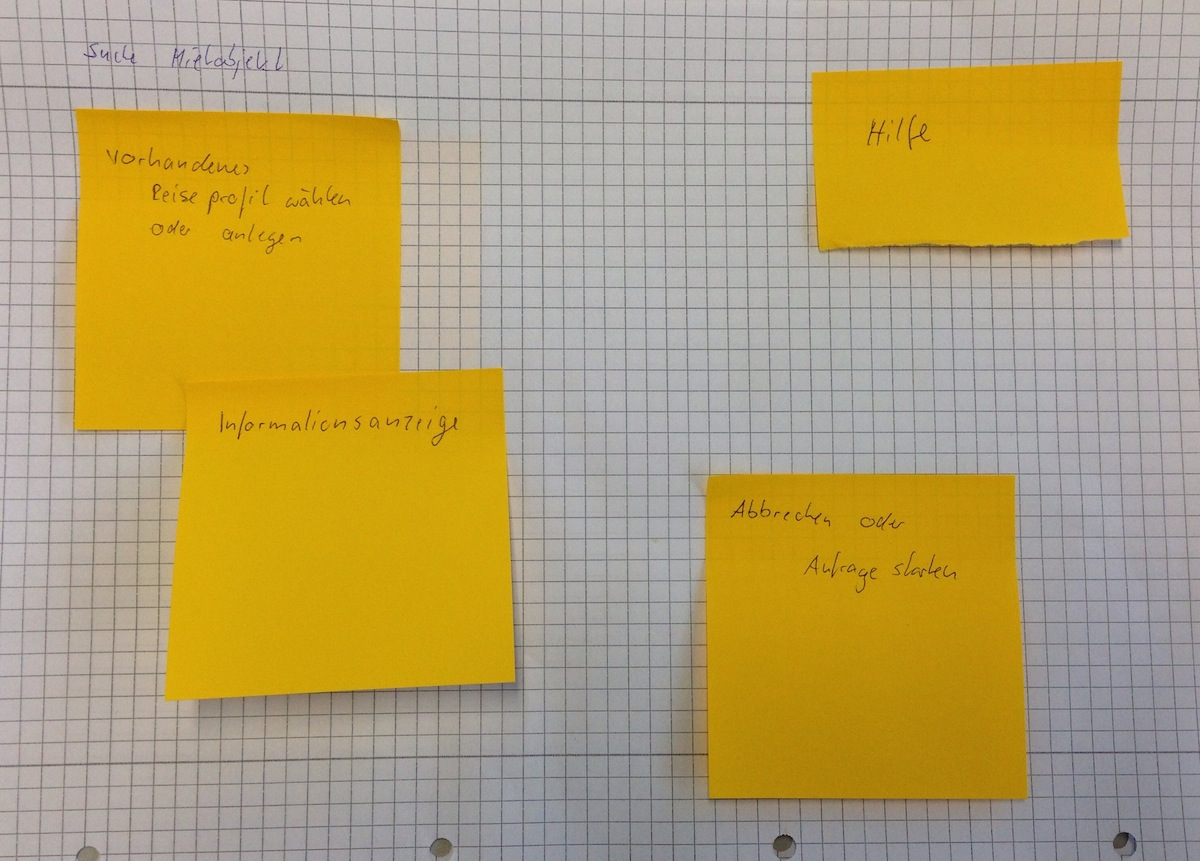
\includegraphics[width=0.85\textwidth]{./images/abstract/version1/sucheMietobjekt.JPG}
\caption{Interaction Context AP1: sucheMietobjekt}
\label{interfaceContents31}
\end{figure}


\chapter{Abstract Prototype 2}

%Seite 1
\begin{figure}[H]
\centering
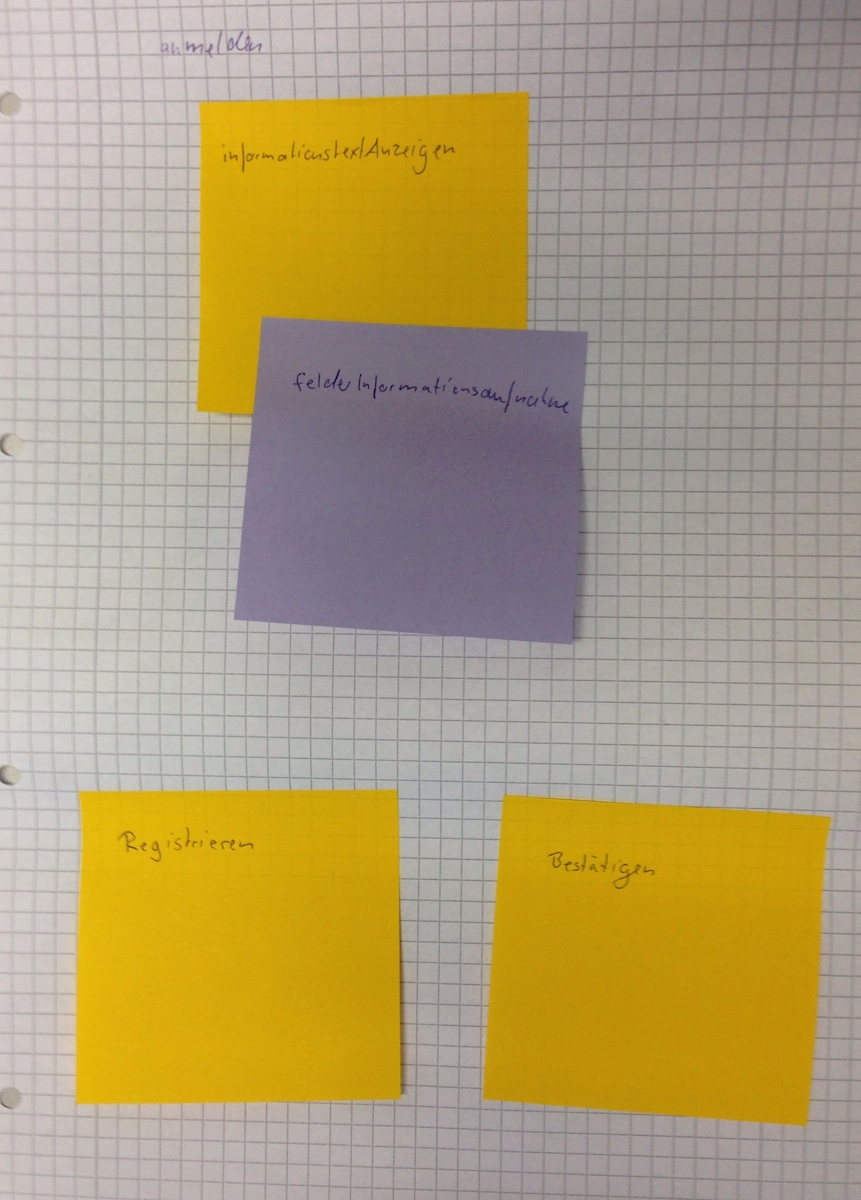
\includegraphics[angle=90, width=0.85\textwidth] {./images/abstract/version2/anmelden.JPG}
\caption{Interaction Context AP2: anmelden}
\label{interfaceContents40}
\end{figure}

\begin{figure}[H]
\centering
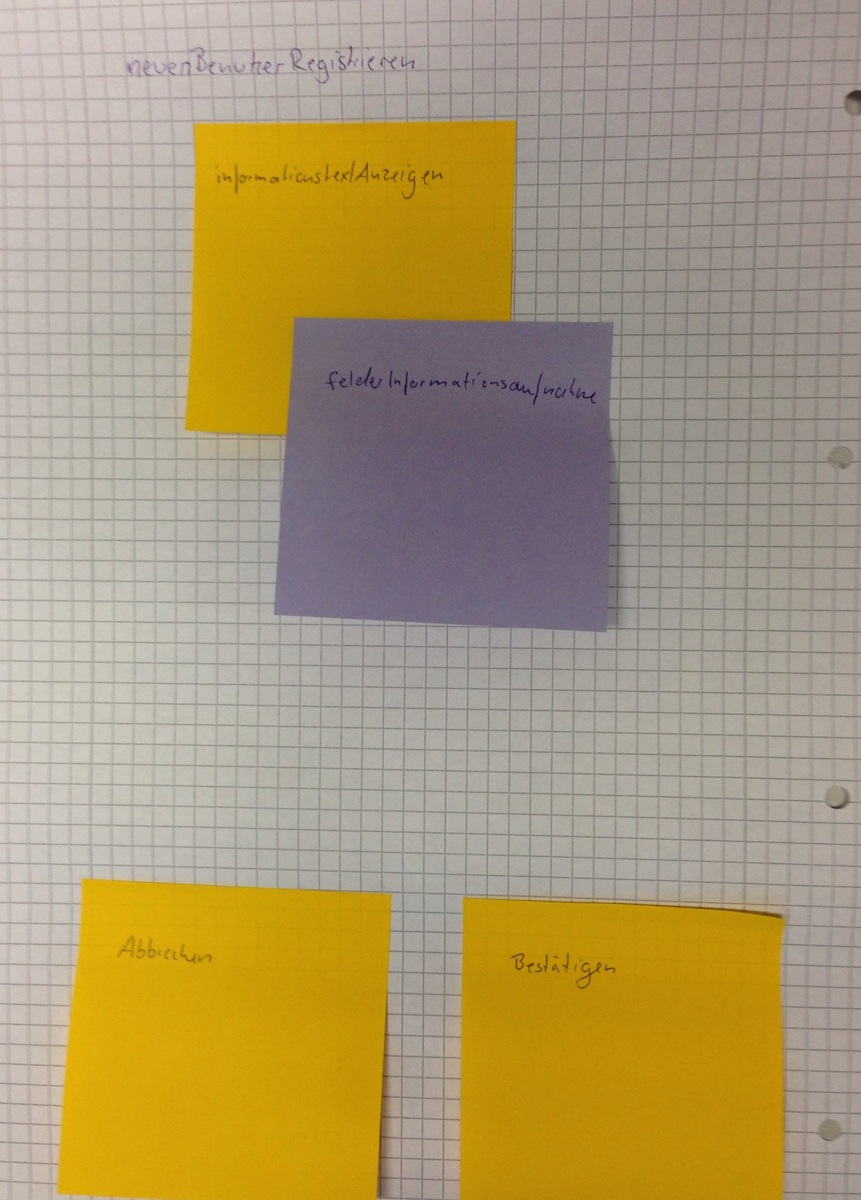
\includegraphics[angle=90, width=0.85\textwidth]  {./images/abstract/version2/neuenBenutzerRegistrieren.JPG}
\caption{Interaction Context AP2: neuenBenutzerRegistrieren}
\label{interfaceContents41}
\end{figure}

%Seite 2
\begin{figure}[H]
\centering
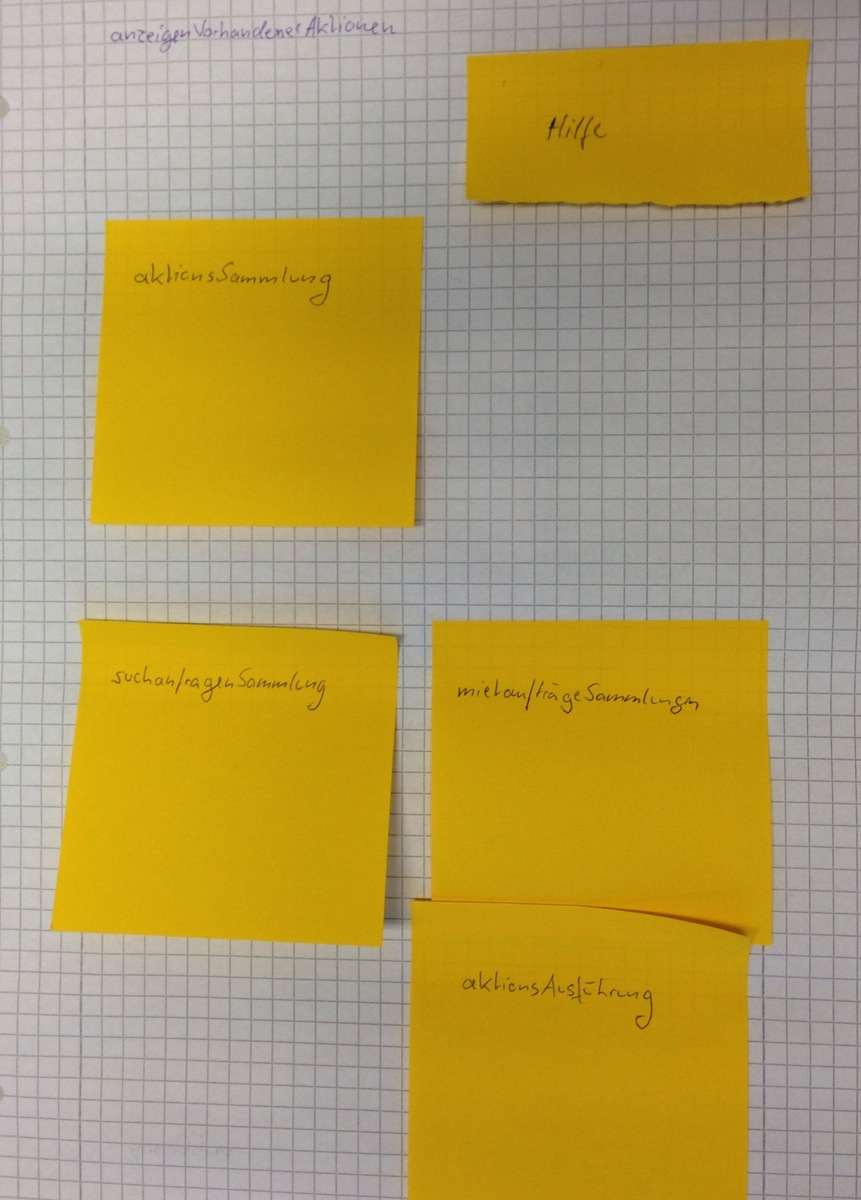
\includegraphics[angle=90, width=0.85\textwidth] {./images/abstract/version2/anzeigenVorhandenerAktionen.JPG}
\caption{Interaction Context AP2: anzeigenVorhandenerAktionen}
\label{interfaceContents42}
\end{figure}

\begin{figure}[H]
\centering
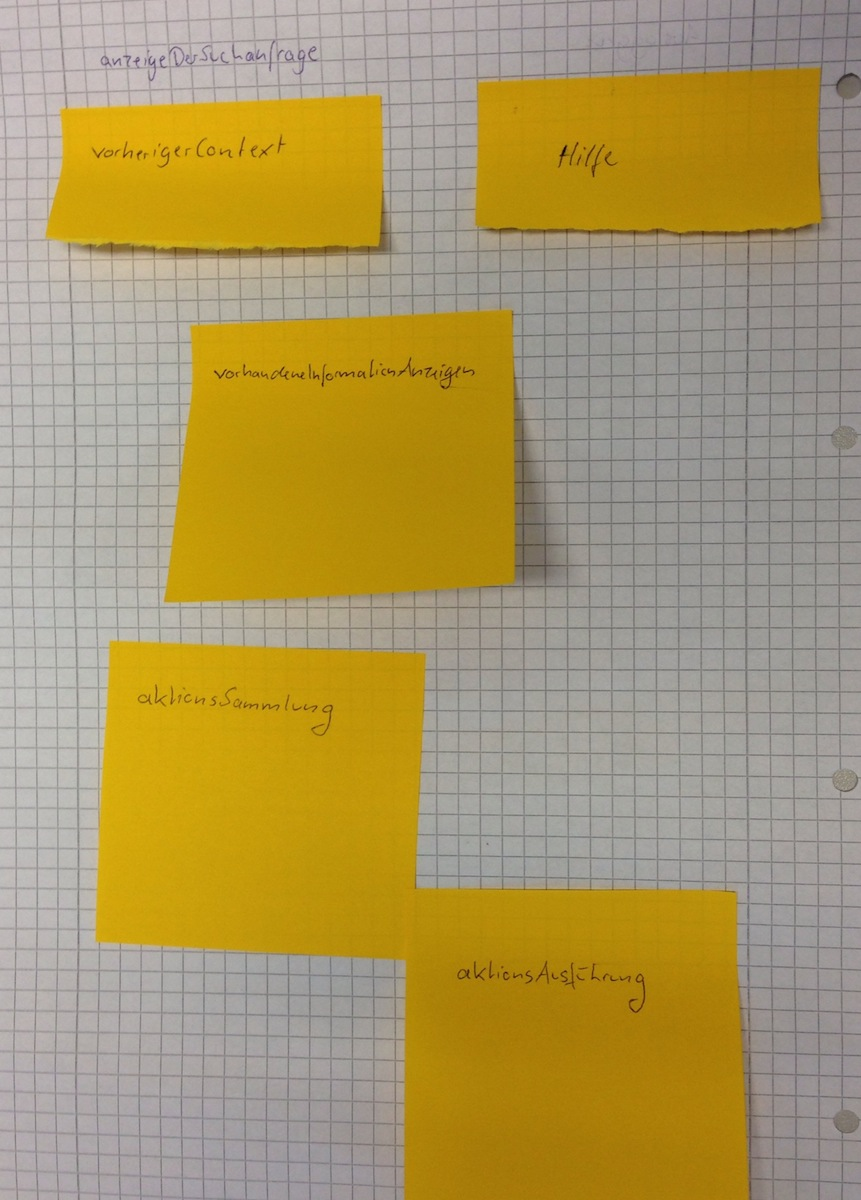
\includegraphics[angle=90, width=0.85\textwidth]  {./images/abstract/version2/anzeigeDerSuchanfrage.JPG}
\caption{Interaction Context AP2: anzeigeDerSuchanfrage}
\label{interfaceContents43}
\end{figure}


%Seite 3
\begin{figure}[H]
\centering
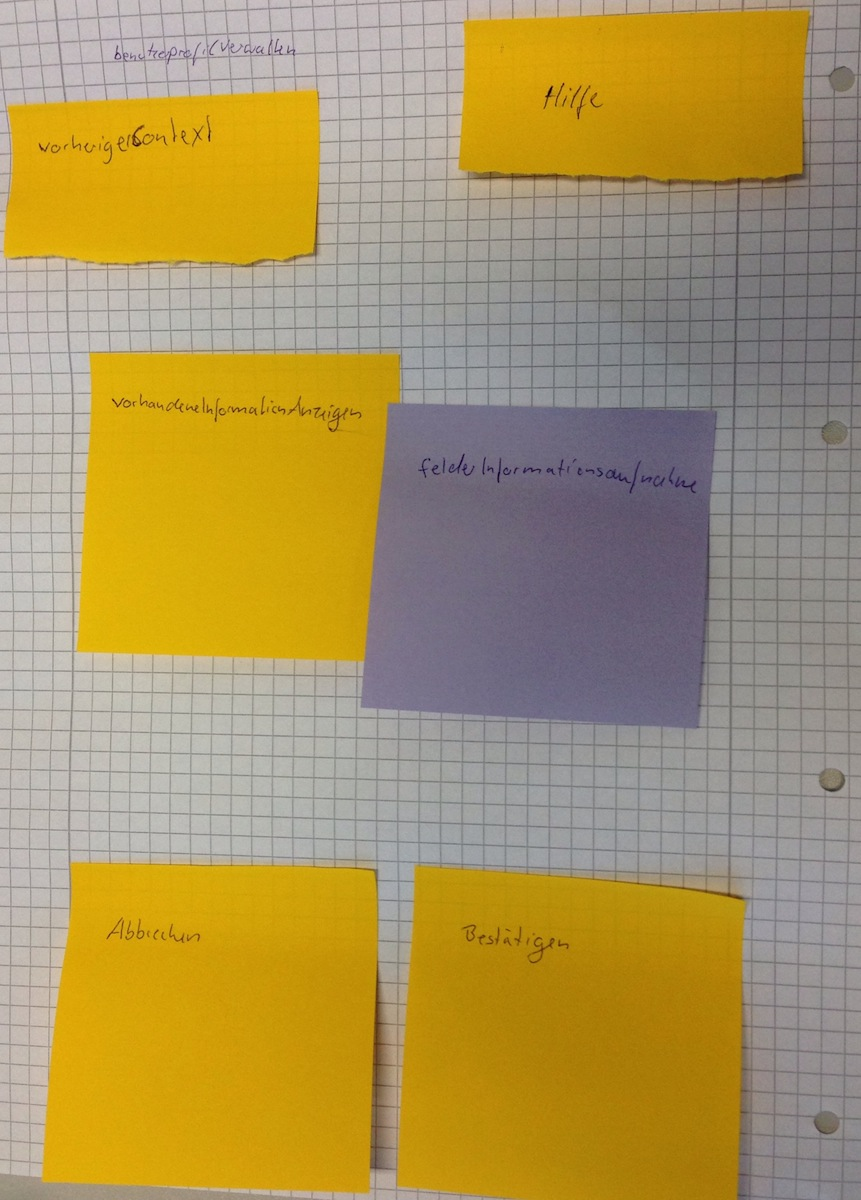
\includegraphics[angle=90, width=0.85\textwidth] {./images/abstract/version2/benutzerprofilVerwalten.JPG}
\caption{Interaction Context AP2: benutzerprofilVerwalten}
\label{interfaceContents44}
\end{figure}

\begin{figure}[H]
\centering
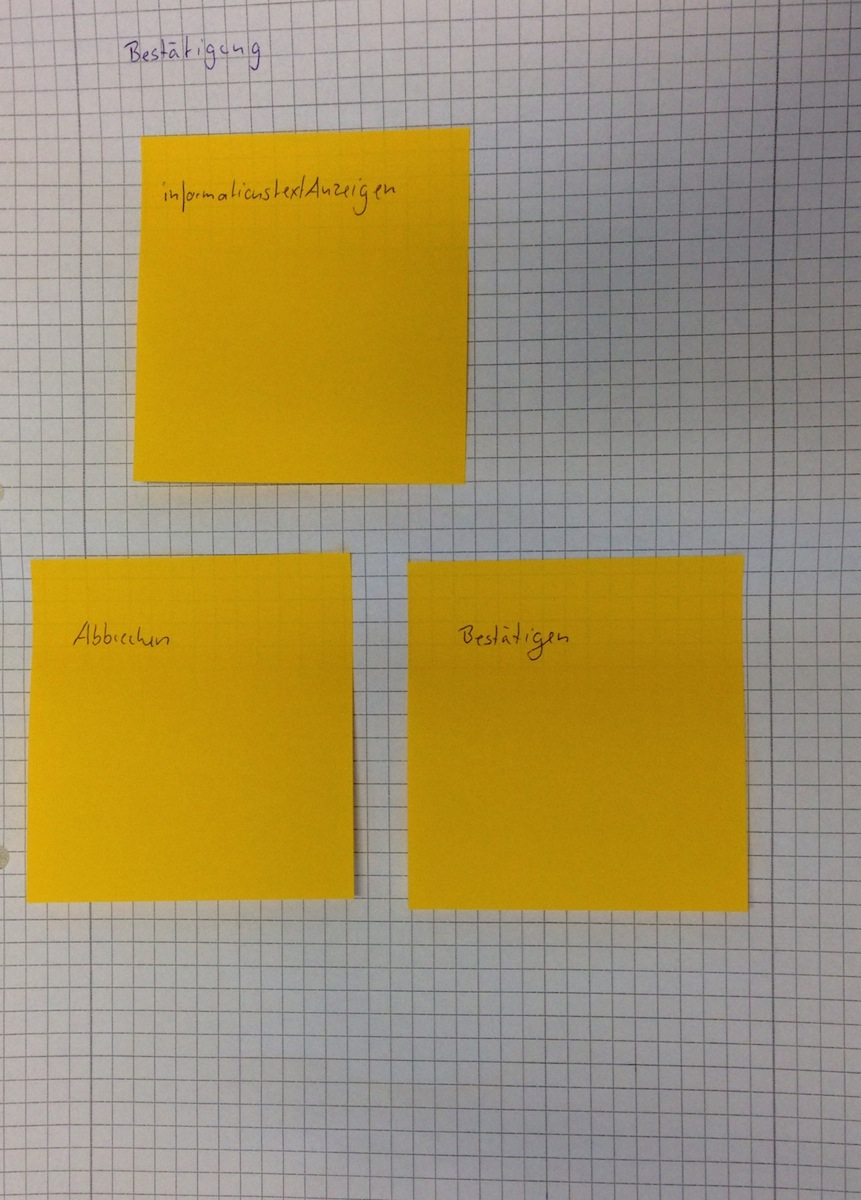
\includegraphics[angle=90, width=0.85\textwidth]  {./images/abstract/version2/bestaetigung.JPG}
\caption{Interaction Context AP2: bestätigung}
\label{interfaceContents45}
\end{figure}


%Seite 4
\begin{figure}[H]
\centering
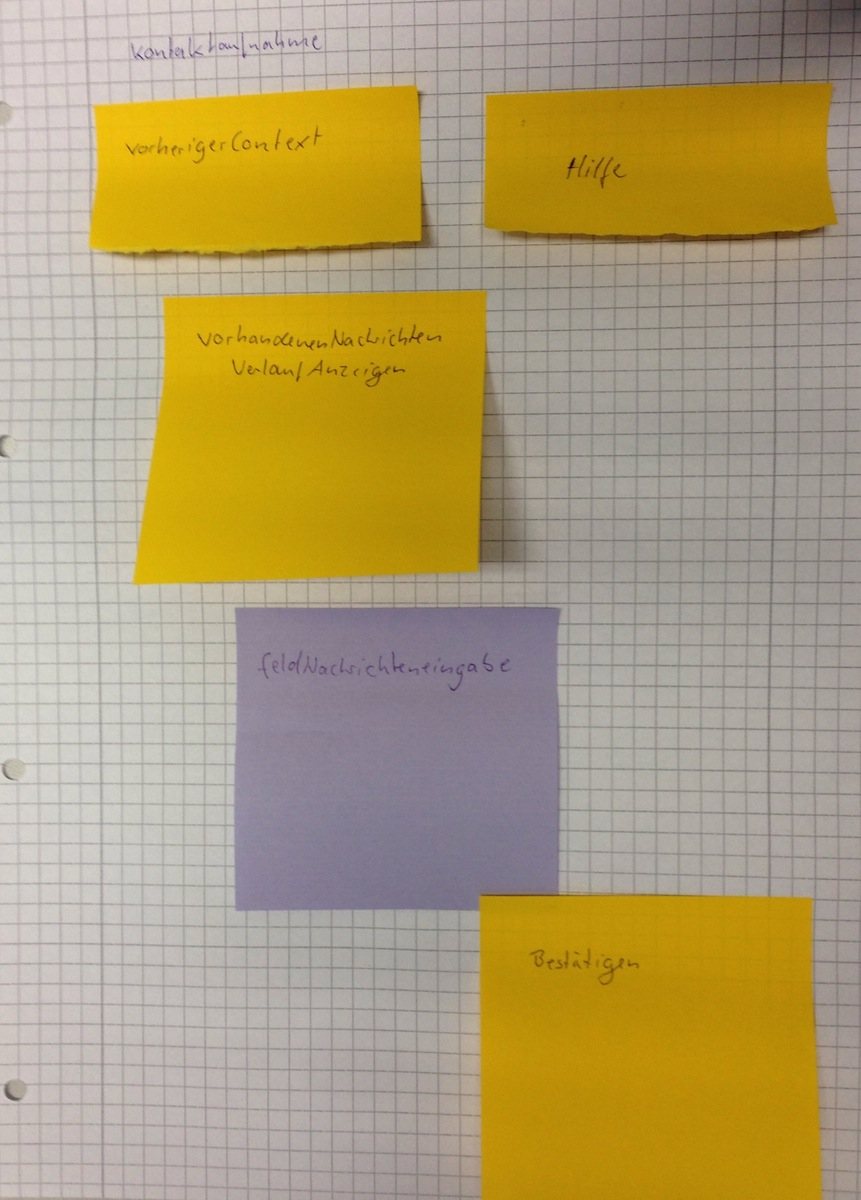
\includegraphics[angle=90, width=0.85\textwidth] {./images/abstract/version2/kontaktaufnahme.JPG}
\caption{Interaction Context AP2: kontaktaufnahme}
\label{interfaceContents46}
\end{figure}

\begin{figure}[H]
\centering
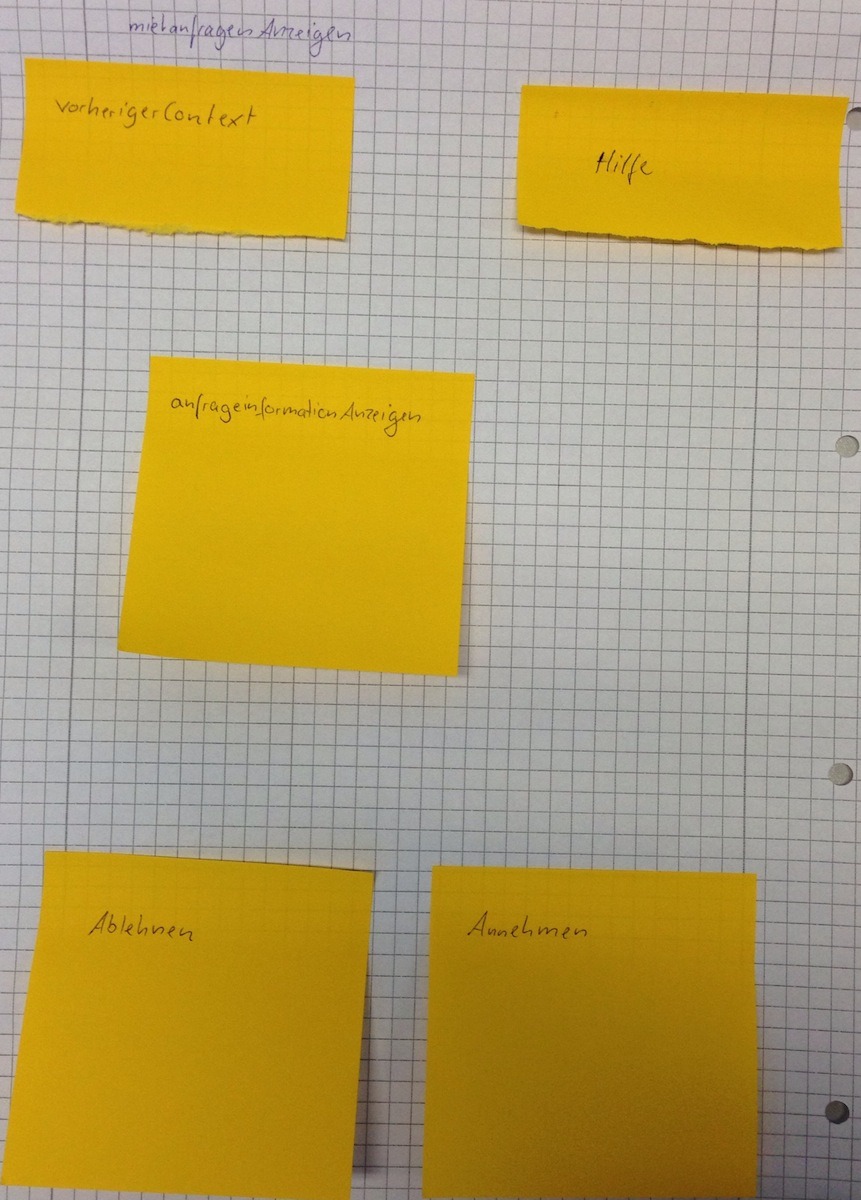
\includegraphics[angle=90, width=0.85\textwidth]  {./images/abstract/version2/mietanfragenAnzeigen.JPG}
\caption{Interaction Context AP2: mietanfragenAnzeigen}
\label{interfaceContents47}
\end{figure}


%Seite 5
\begin{figure}[H]
\centering
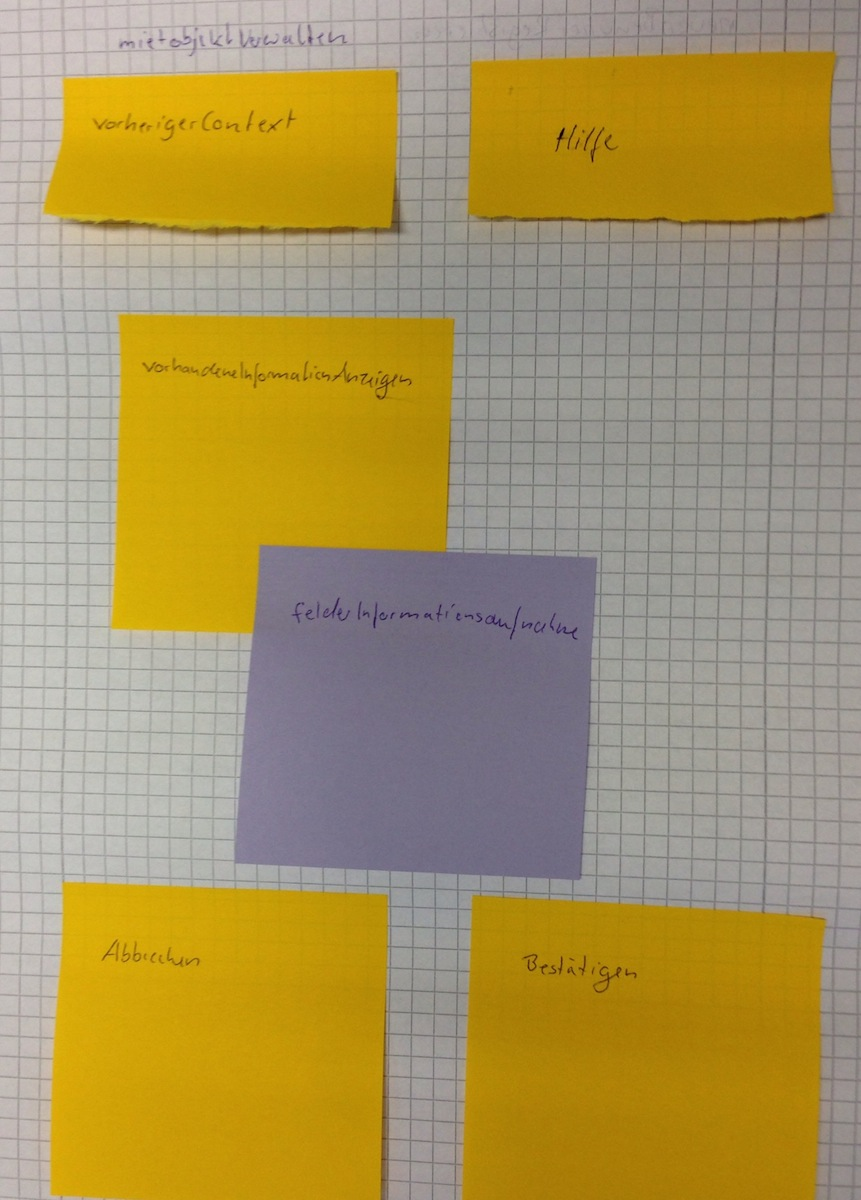
\includegraphics[angle=90, width=0.85\textwidth] {./images/abstract/version2/mietobjekteVerwalten.JPG}
\caption{Interaction Context AP2: mietobjekteVerwalten}
\label{interfaceContents48}
\end{figure}

\begin{figure}[H]
\centering
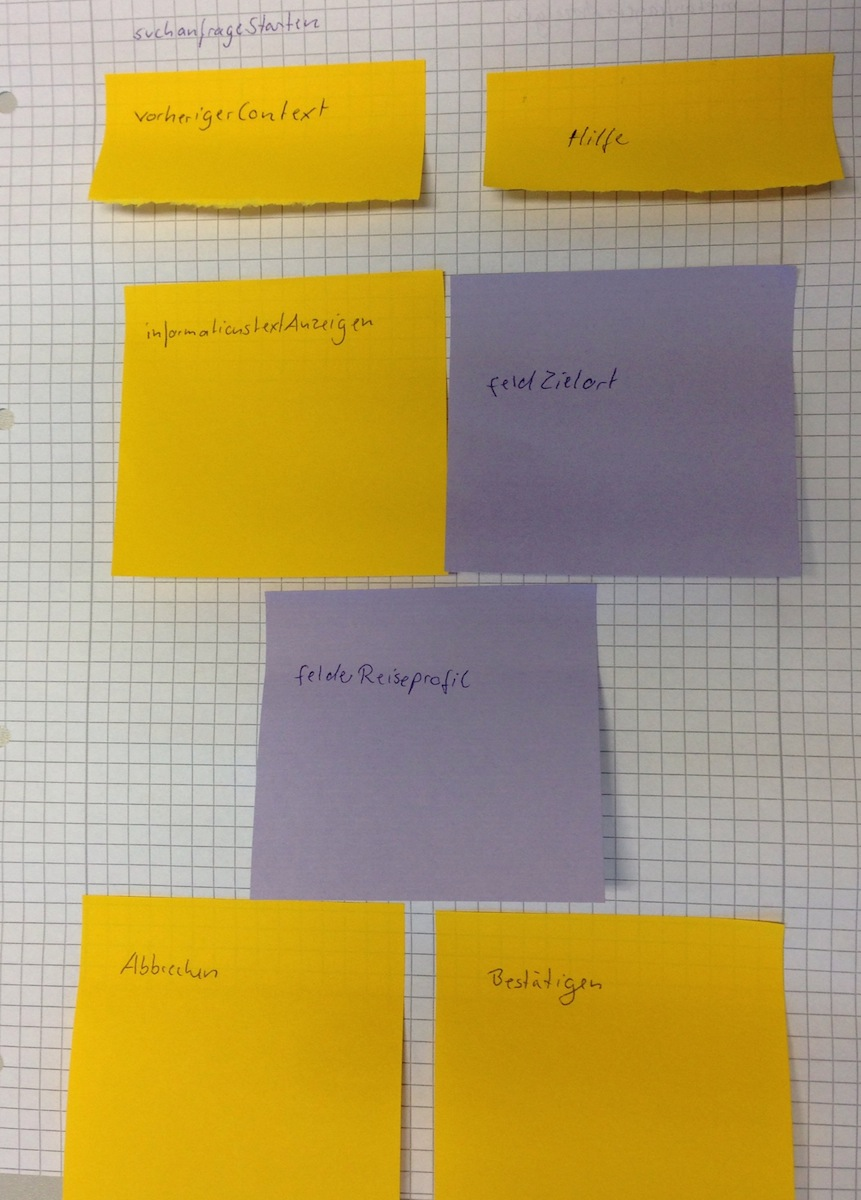
\includegraphics[angle=90, width=0.85\textwidth]  {./images/abstract/version2/suchanfragenStarten.JPG}
\caption{Interaction Context AP2: suchanfrageStarten}
\label{interfaceContents49}
\end{figure}


%Seite 6
\begin{figure}[H]
\centering
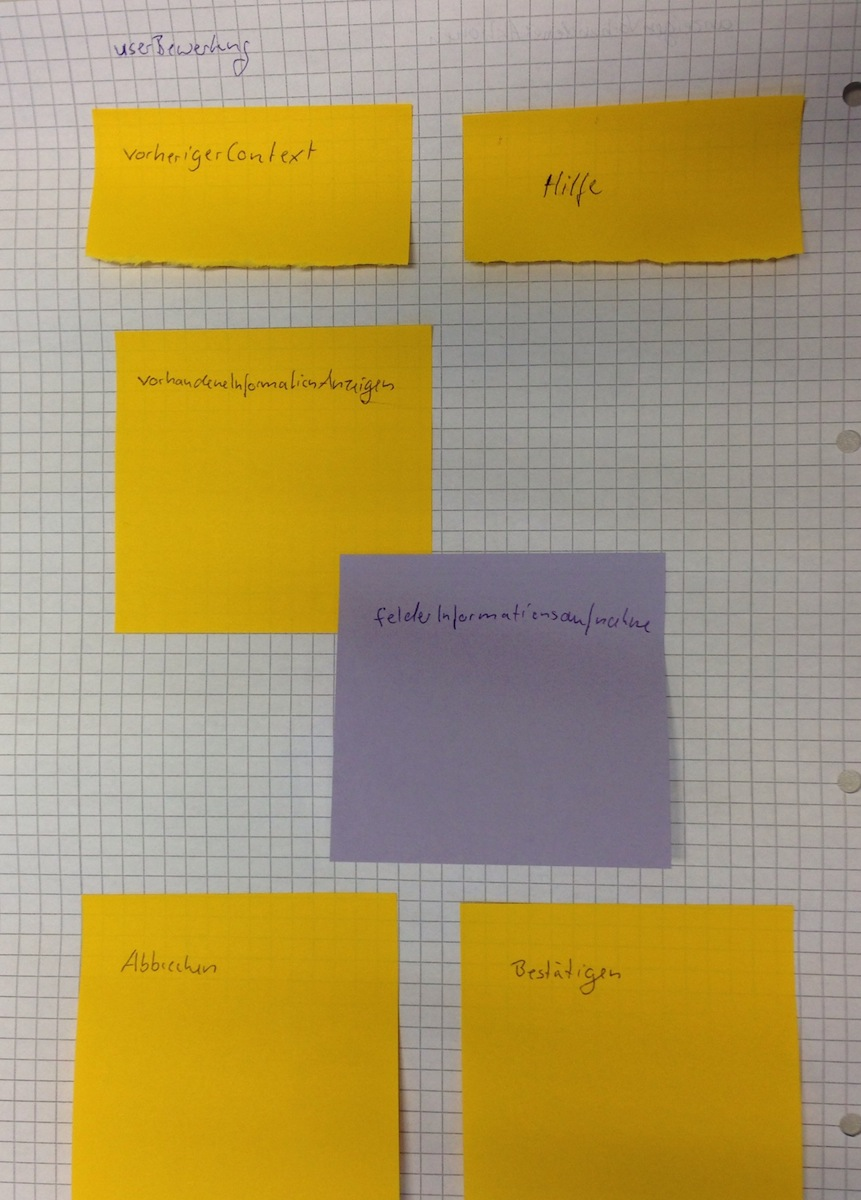
\includegraphics[angle=90, width=0.85\textwidth] {./images/abstract/version2/userBewertung.JPG}
\caption{Interaction Context AP2: userBewertung}
\label{interfaceContents50}
\end{figure}

\begin{figure}[H]
\centering
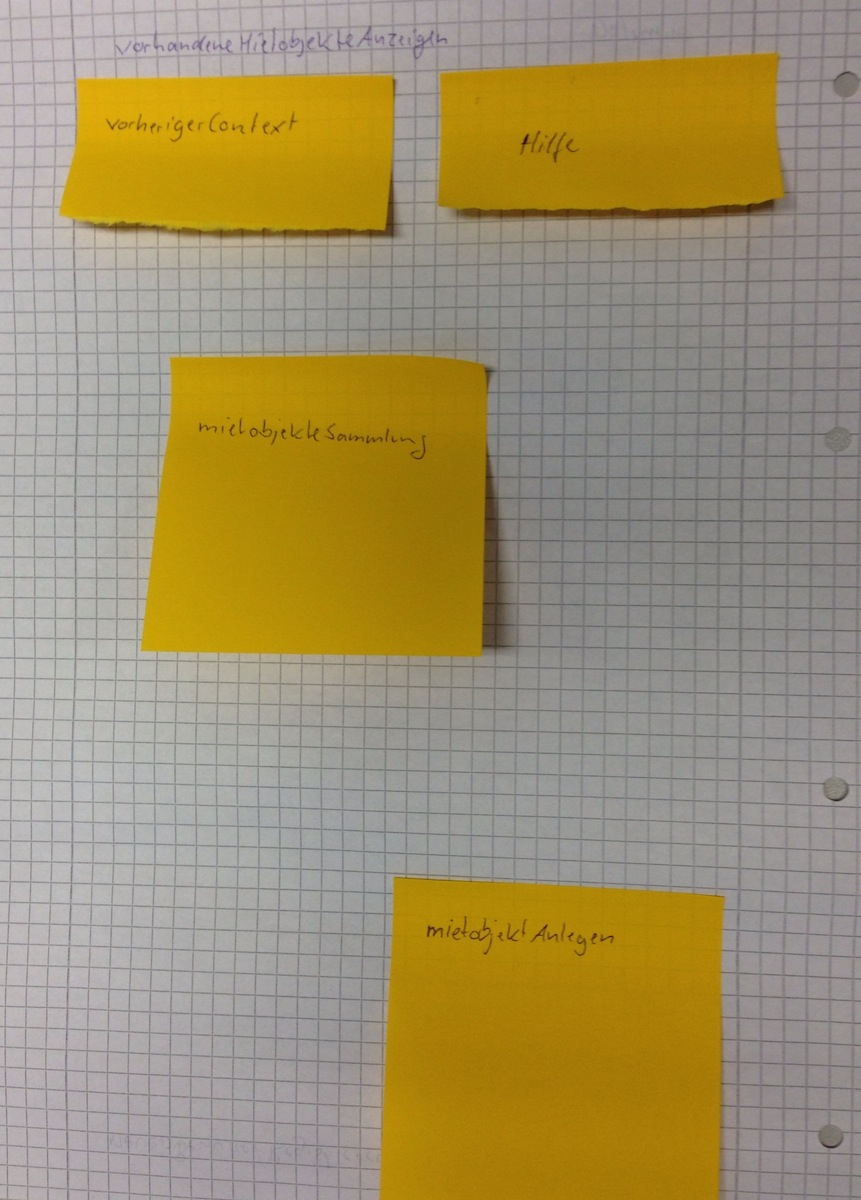
\includegraphics[angle=90, width=0.85\textwidth]  {./images/abstract/version2/vorhandeneMietobjekteAnzeigen.JPG}
\caption{Interaction Context AP2: vorhandeneMietobjekteAnzeigen}
\label{interfaceContents51}
\end{figure}


%Seite 7
\begin{figure}[H]
\centering
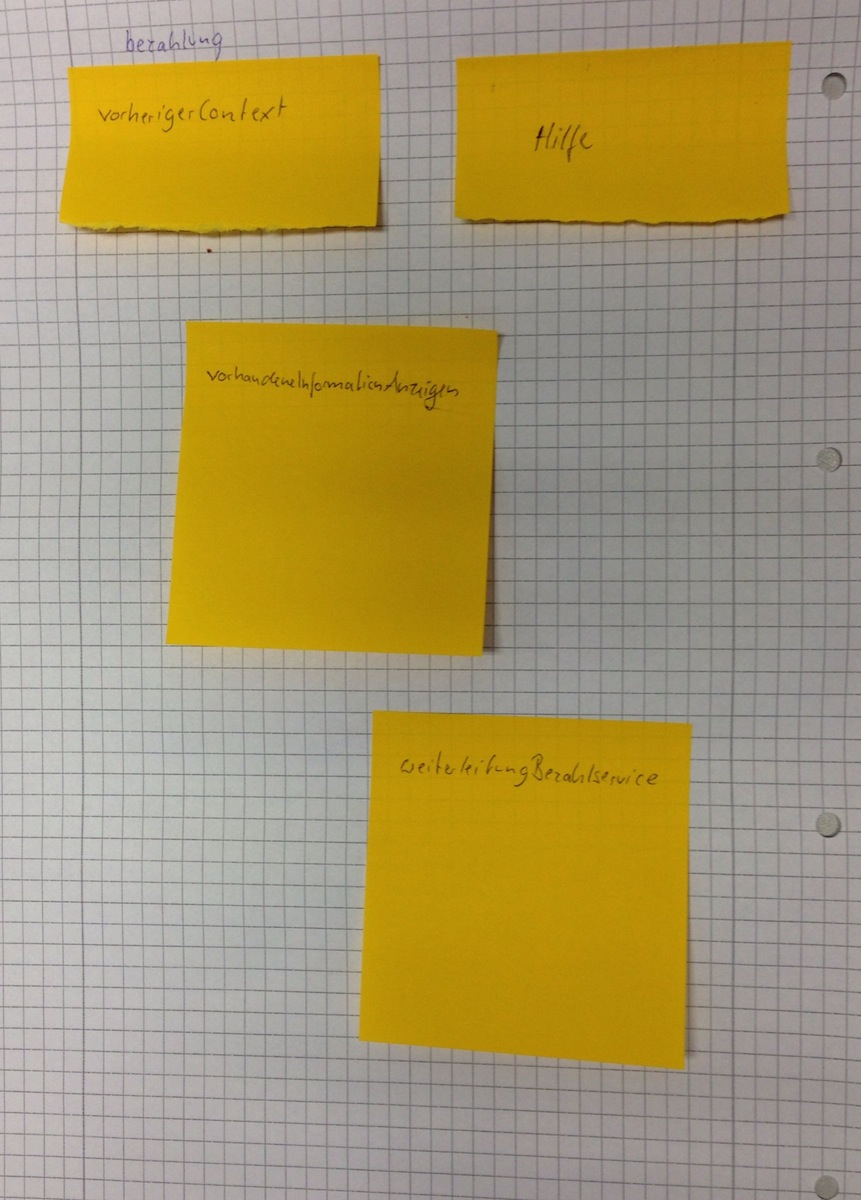
\includegraphics[angle=90, width=0.85\textwidth] {./images/abstract/version2/bezahlung.JPG}
\caption{Interaction Context AP2: bezahlung}
\label{interfaceContents52}
\end{figure}


\chapter{Paperbased Prototype 1}

\begin{figure}[H]
\centering
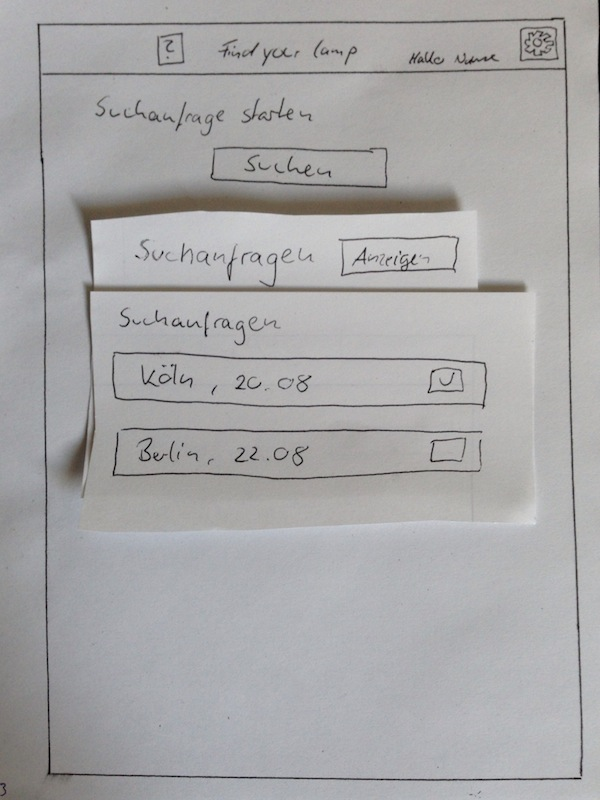
\includegraphics[angle=90, width=0.85\textwidth]{./images/paperbased/anfrage.JPG}
\caption{Pb Prototype: Übersicht der Suchanfragen}
\label{pbprototype1}
\end{figure}

\begin{figure}[H]
\centering
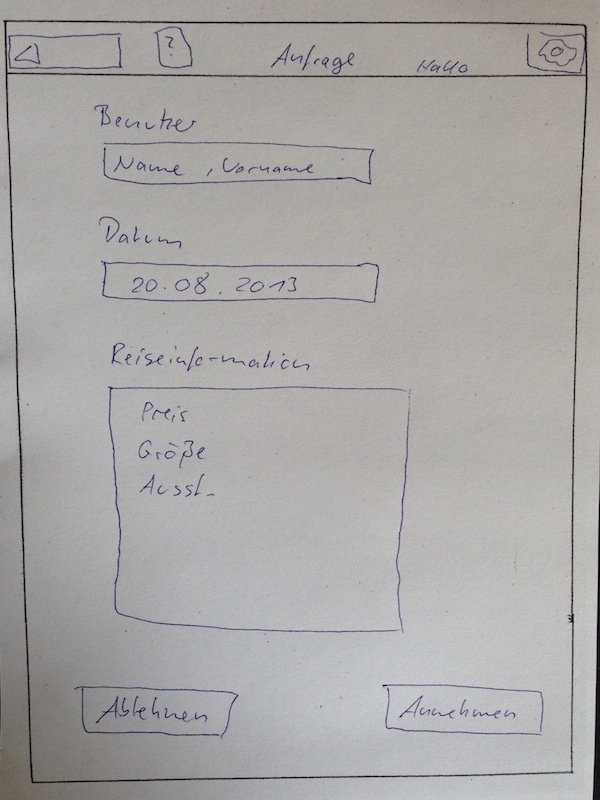
\includegraphics[angle=90, width=0.85\textwidth]{./images/paperbased/anfrageAnzeigen.JPG}
\caption{Pb Prototype: Neue Mietanfrage anzeigen}
\label{pbprototype2}
\end{figure}

\begin{figure}[H]
\centering
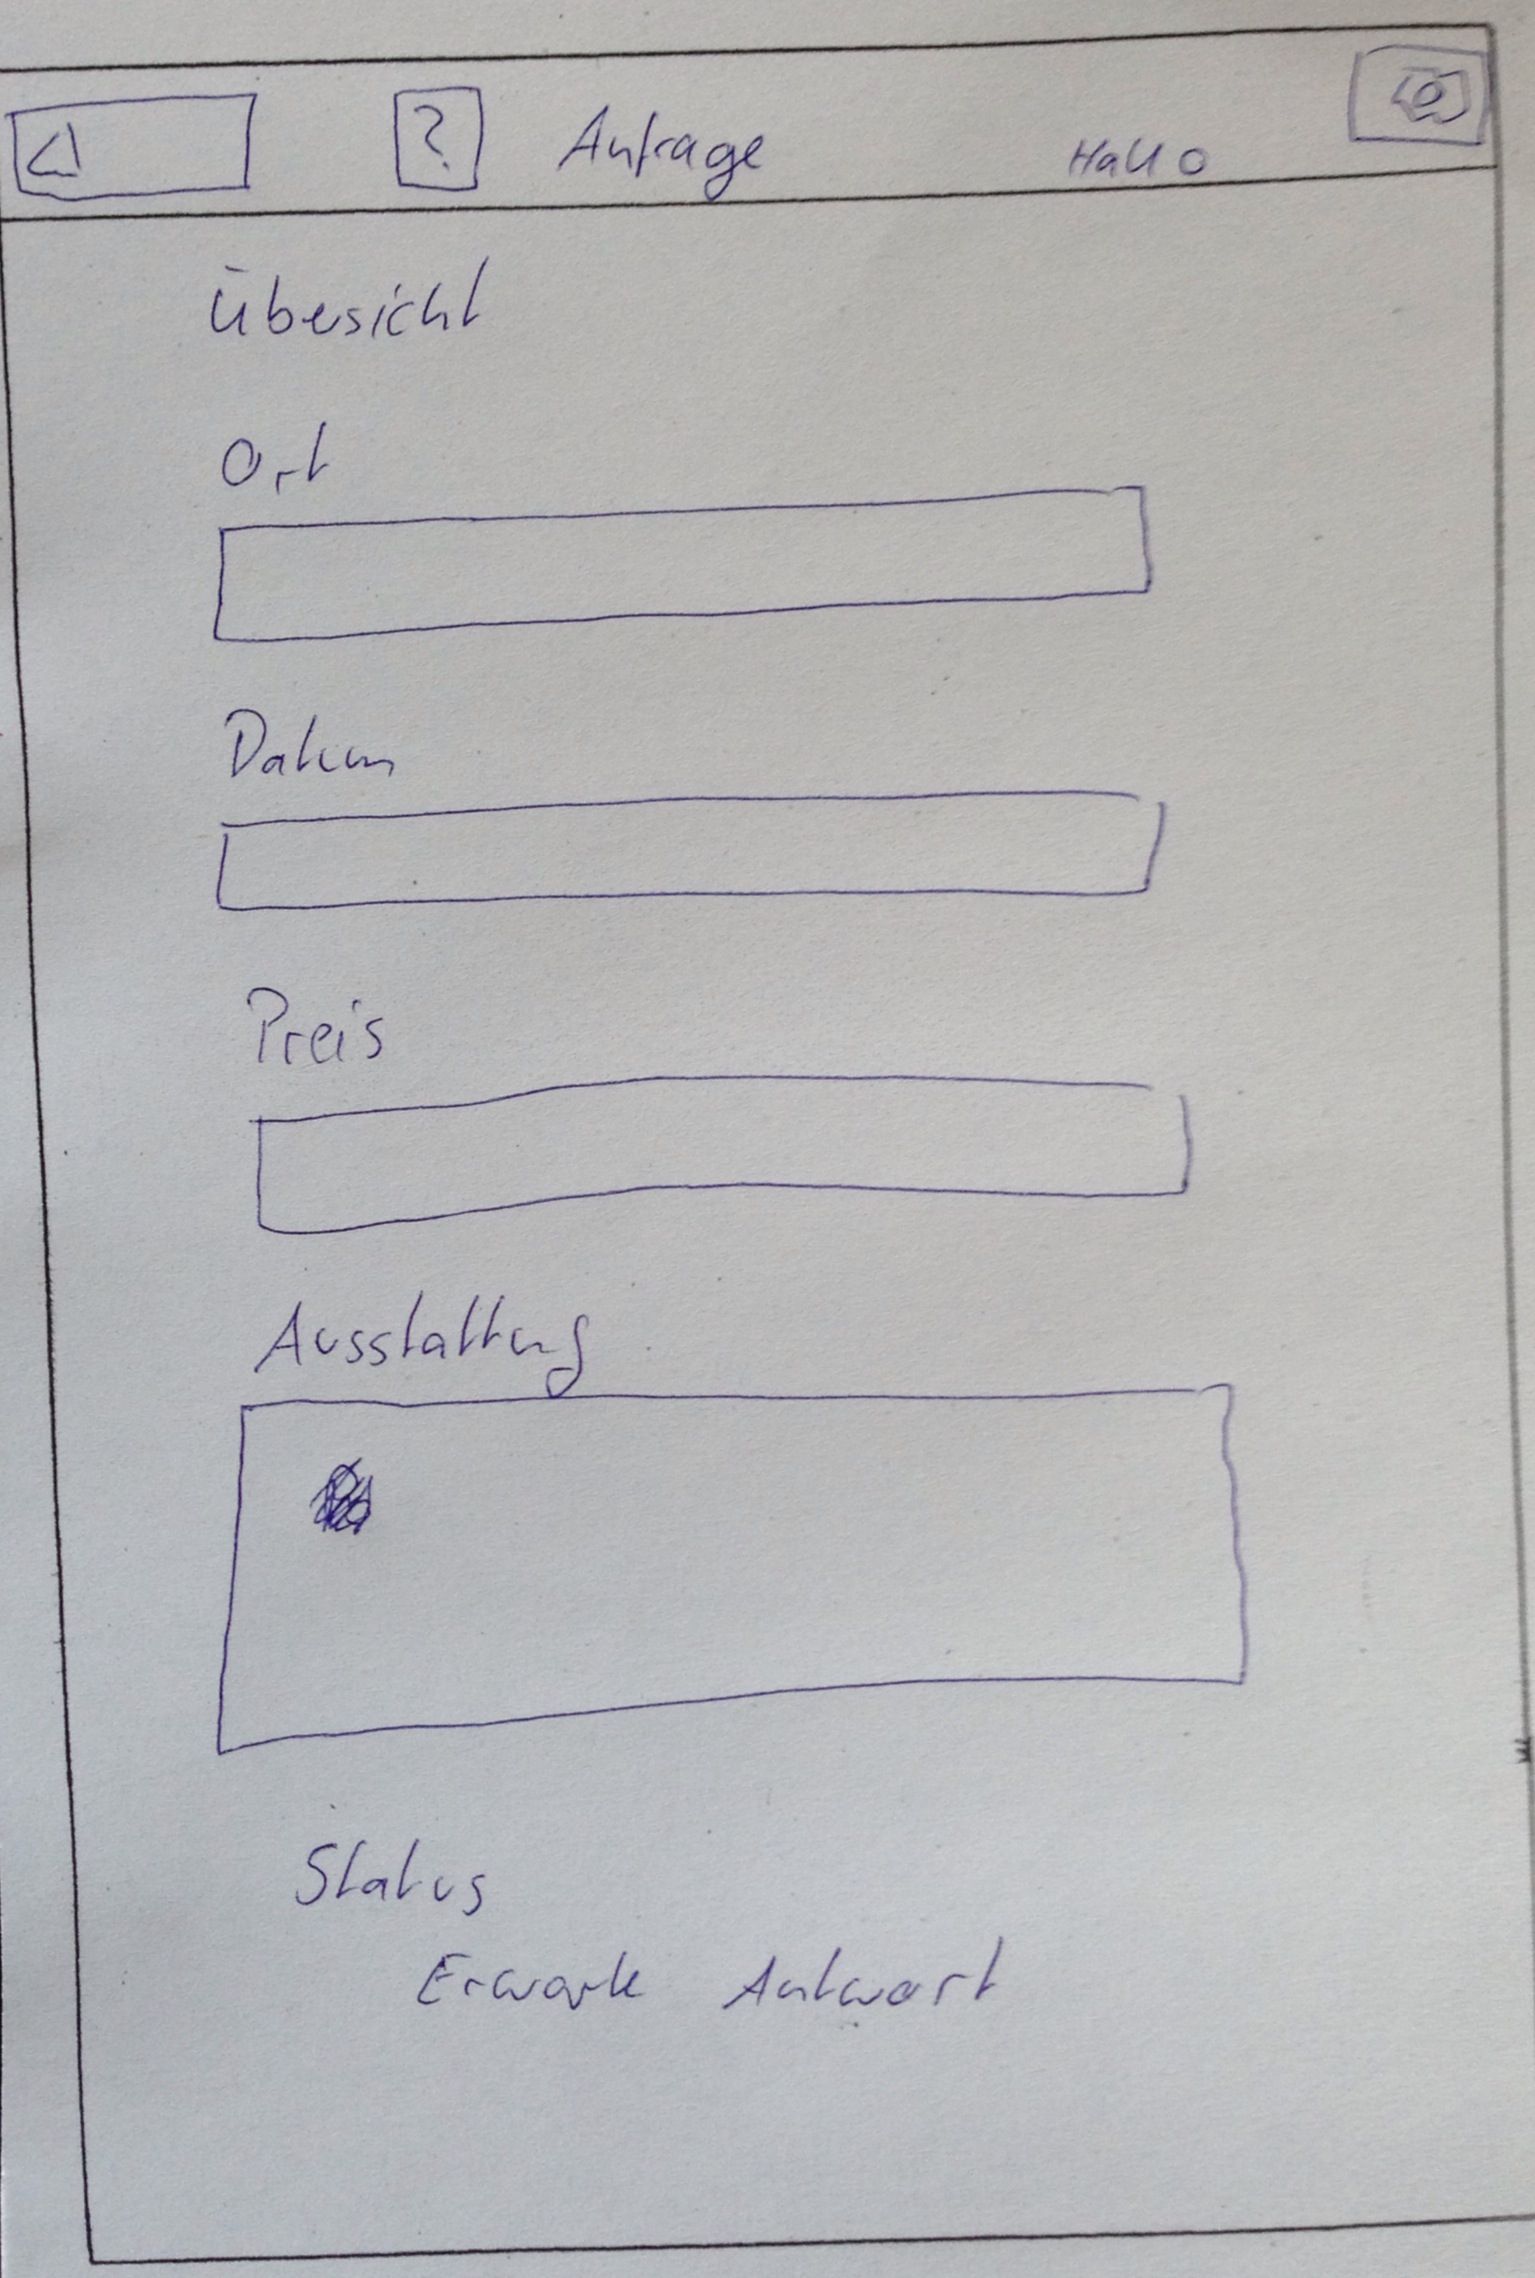
\includegraphics[angle=90, width=0.85\textwidth]{./images/paperbased/anfrageuebersicht.JPG}
\caption{Pb Prototype: Übersicht der Mietanfrage}
\label{pbprototype3}
\end{figure}

\begin{figure}[H]
\centering
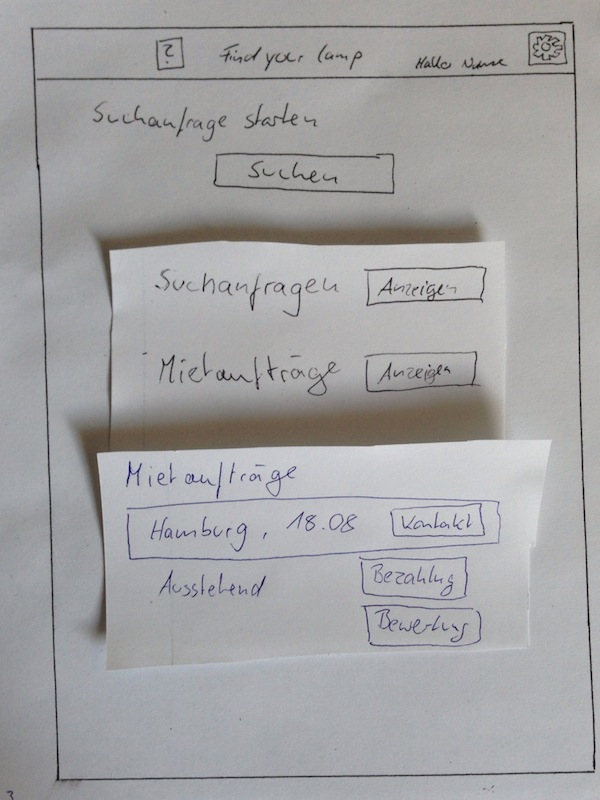
\includegraphics[angle=90, width=0.85\textwidth]{./images/paperbased/auftraege.JPG}
\caption{Pb Prototype: Übersicht der Aufträge}
\label{pbprototype4}
\end{figure}

\begin{figure}[H]
\centering
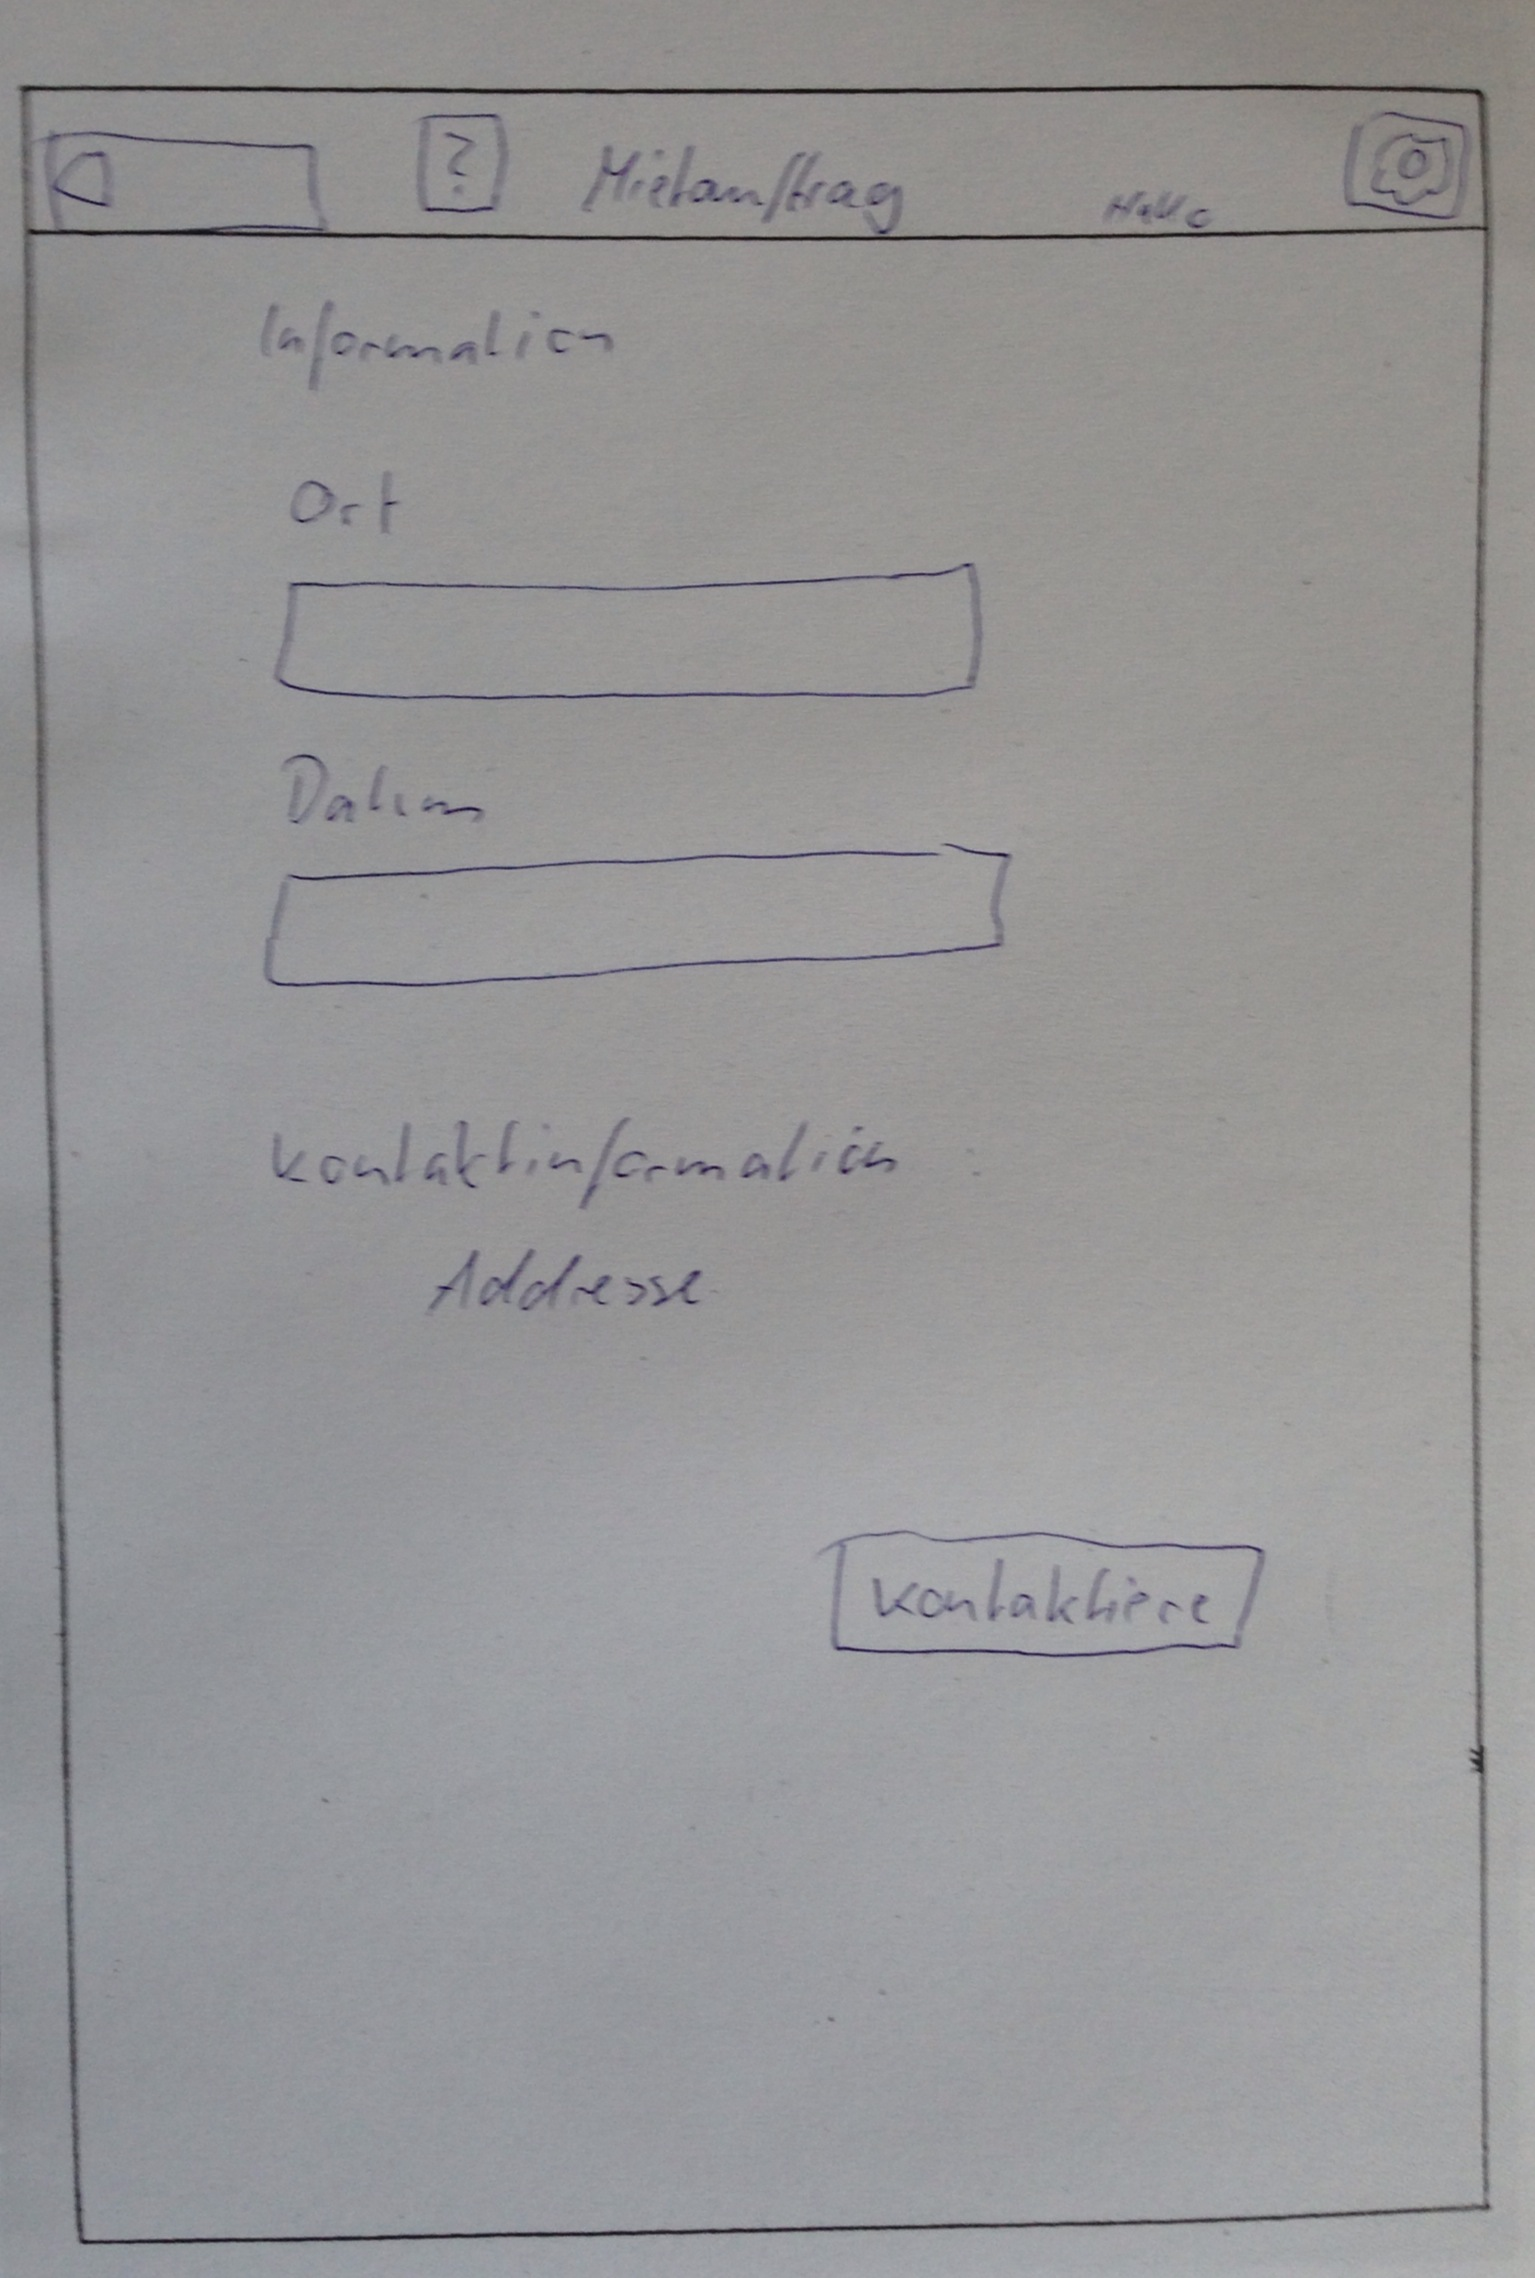
\includegraphics[angle=90, width=0.85\textwidth]{./images/paperbased/auftrag.JPG}
\caption{Pb Prototype: Übersicht eines Mietauftrags}
\label{pbprototype5}
\end{figure}

\begin{figure}[H]
\centering
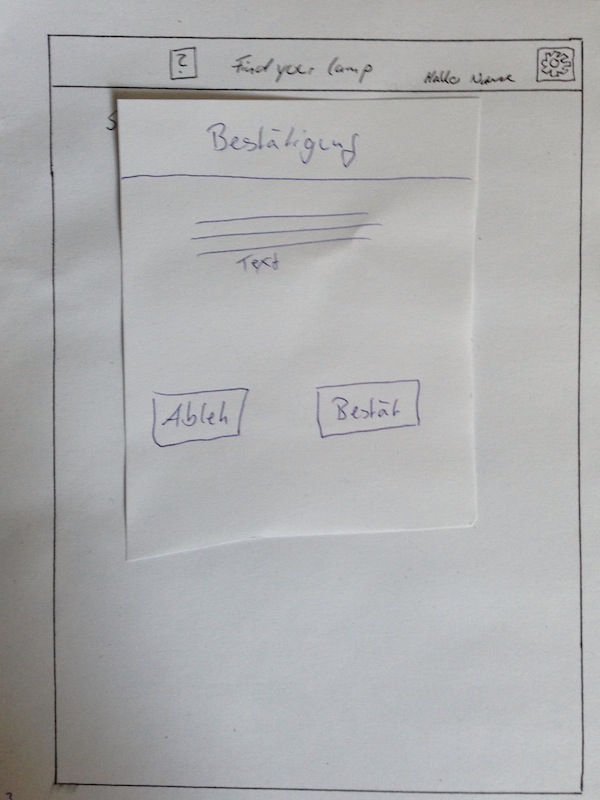
\includegraphics[angle=90, width=0.85\textwidth]{./images/paperbased/bestaetigung.JPG}
\caption{Pb Prototype: Bestätigungsnachricht}
\label{pbprototype6}
\end{figure}

\begin{figure}[H]
\centering
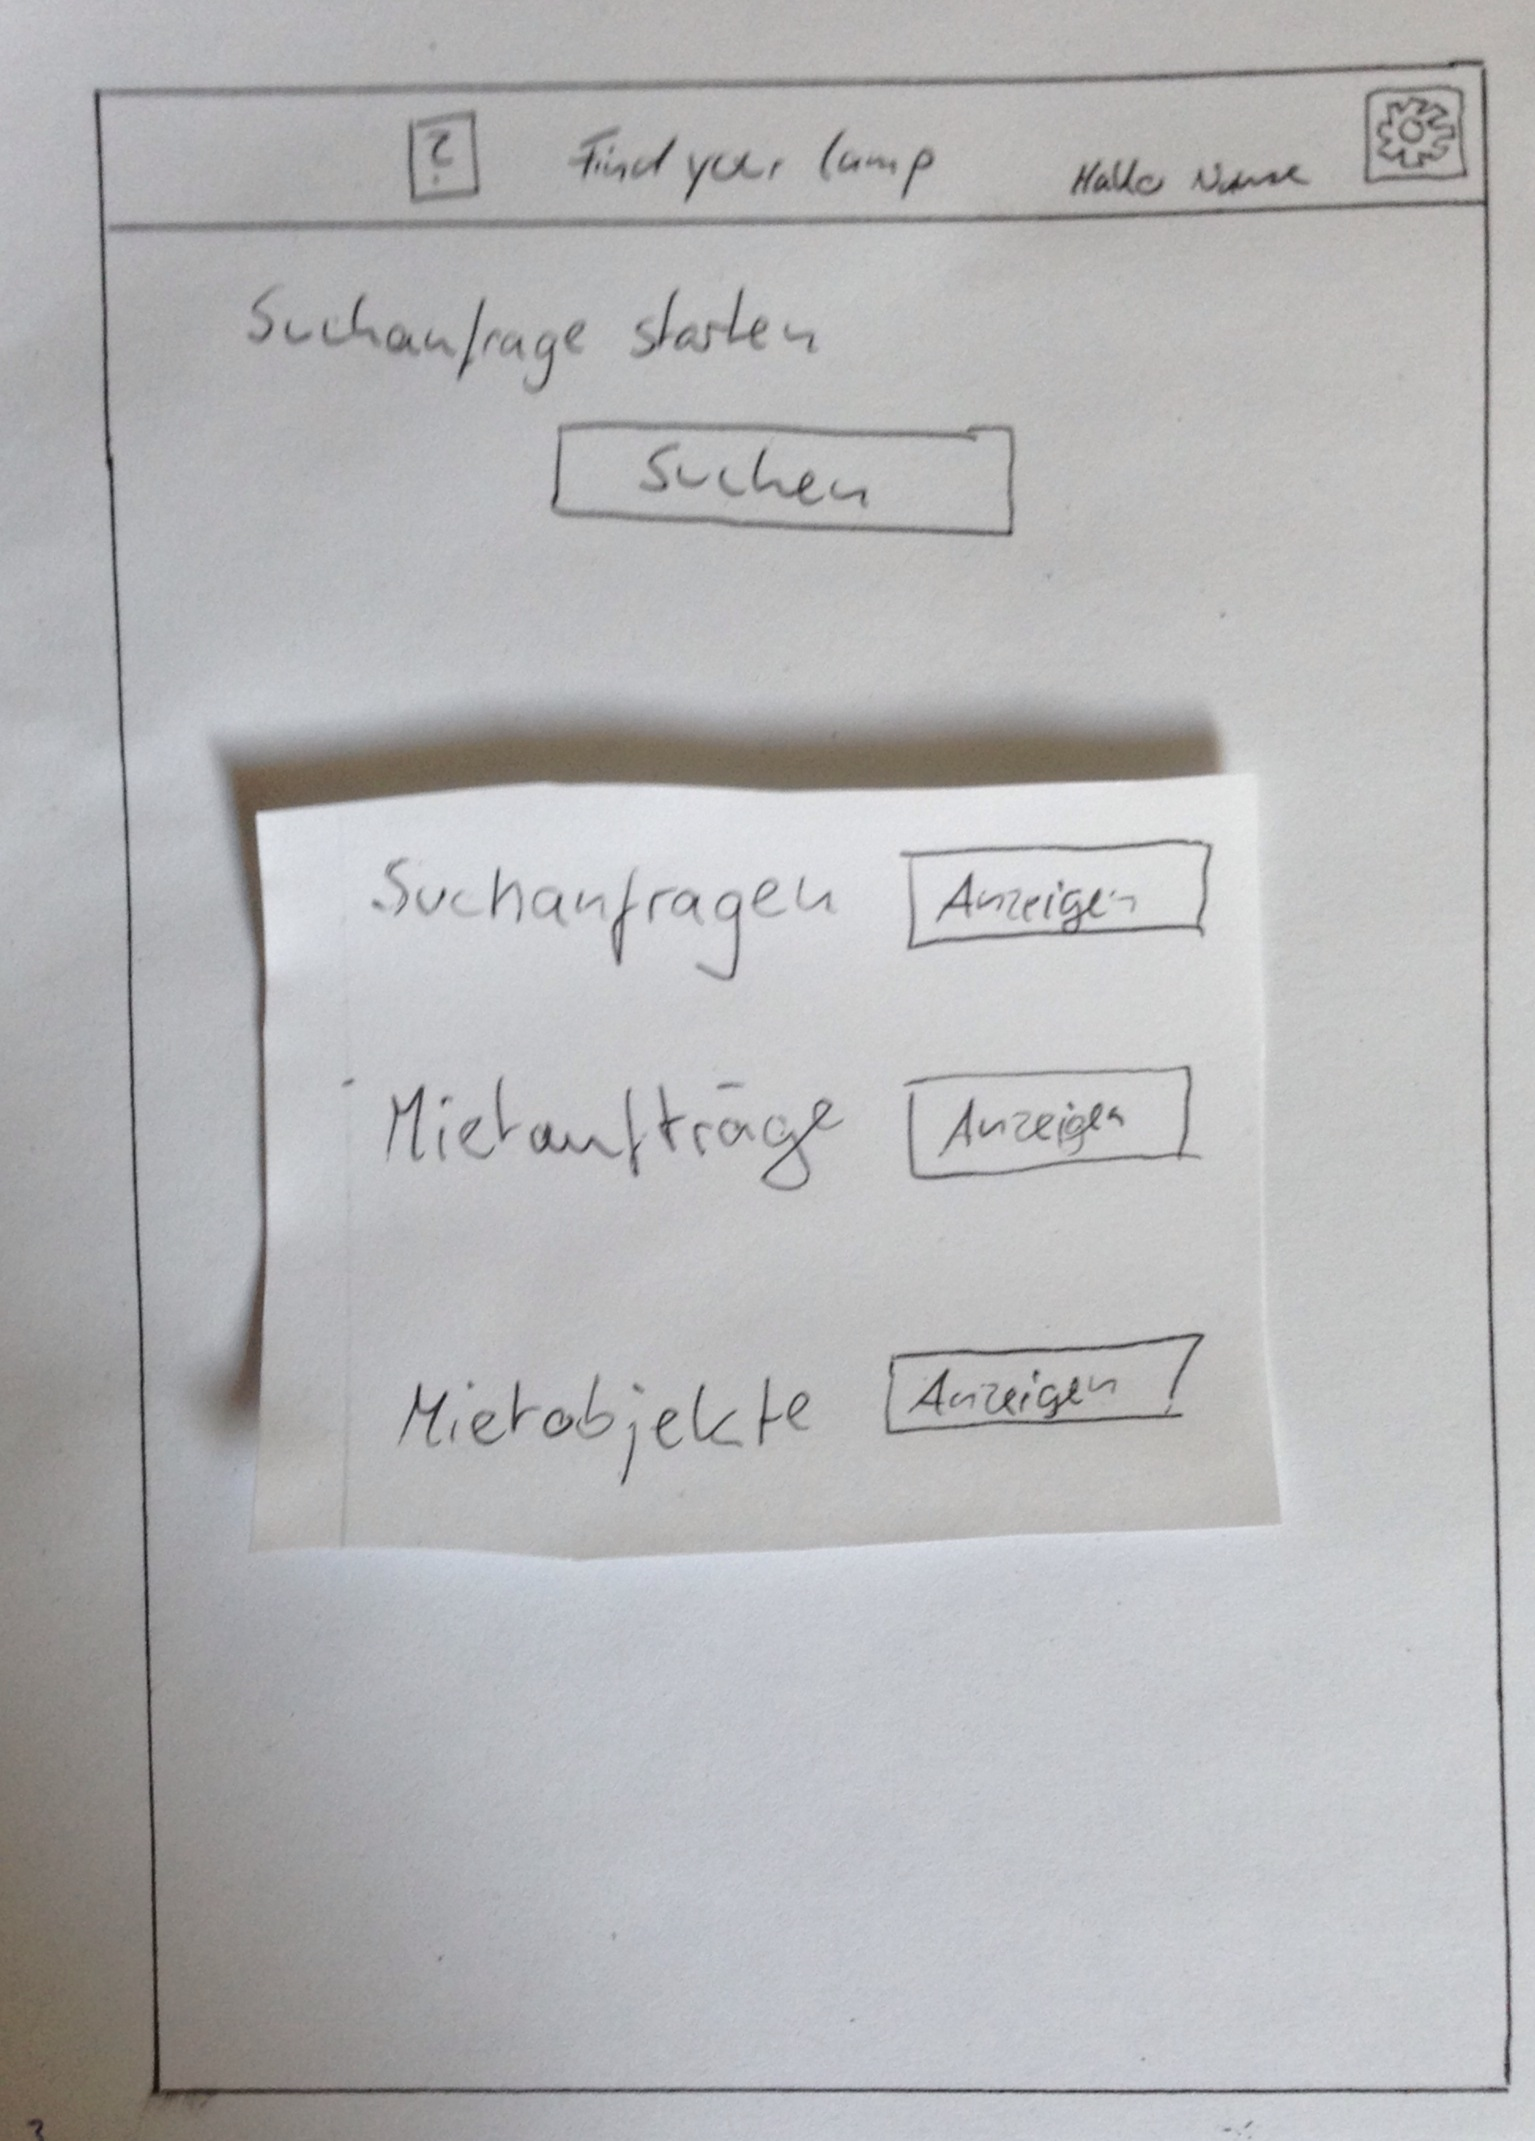
\includegraphics[angle=90, width=0.85\textwidth]{./images/paperbased/main.JPG}
\caption{Pb Prototype: Hauptscreen}
\label{pbprototype7}
\end{figure}

\begin{figure}[H]
\centering
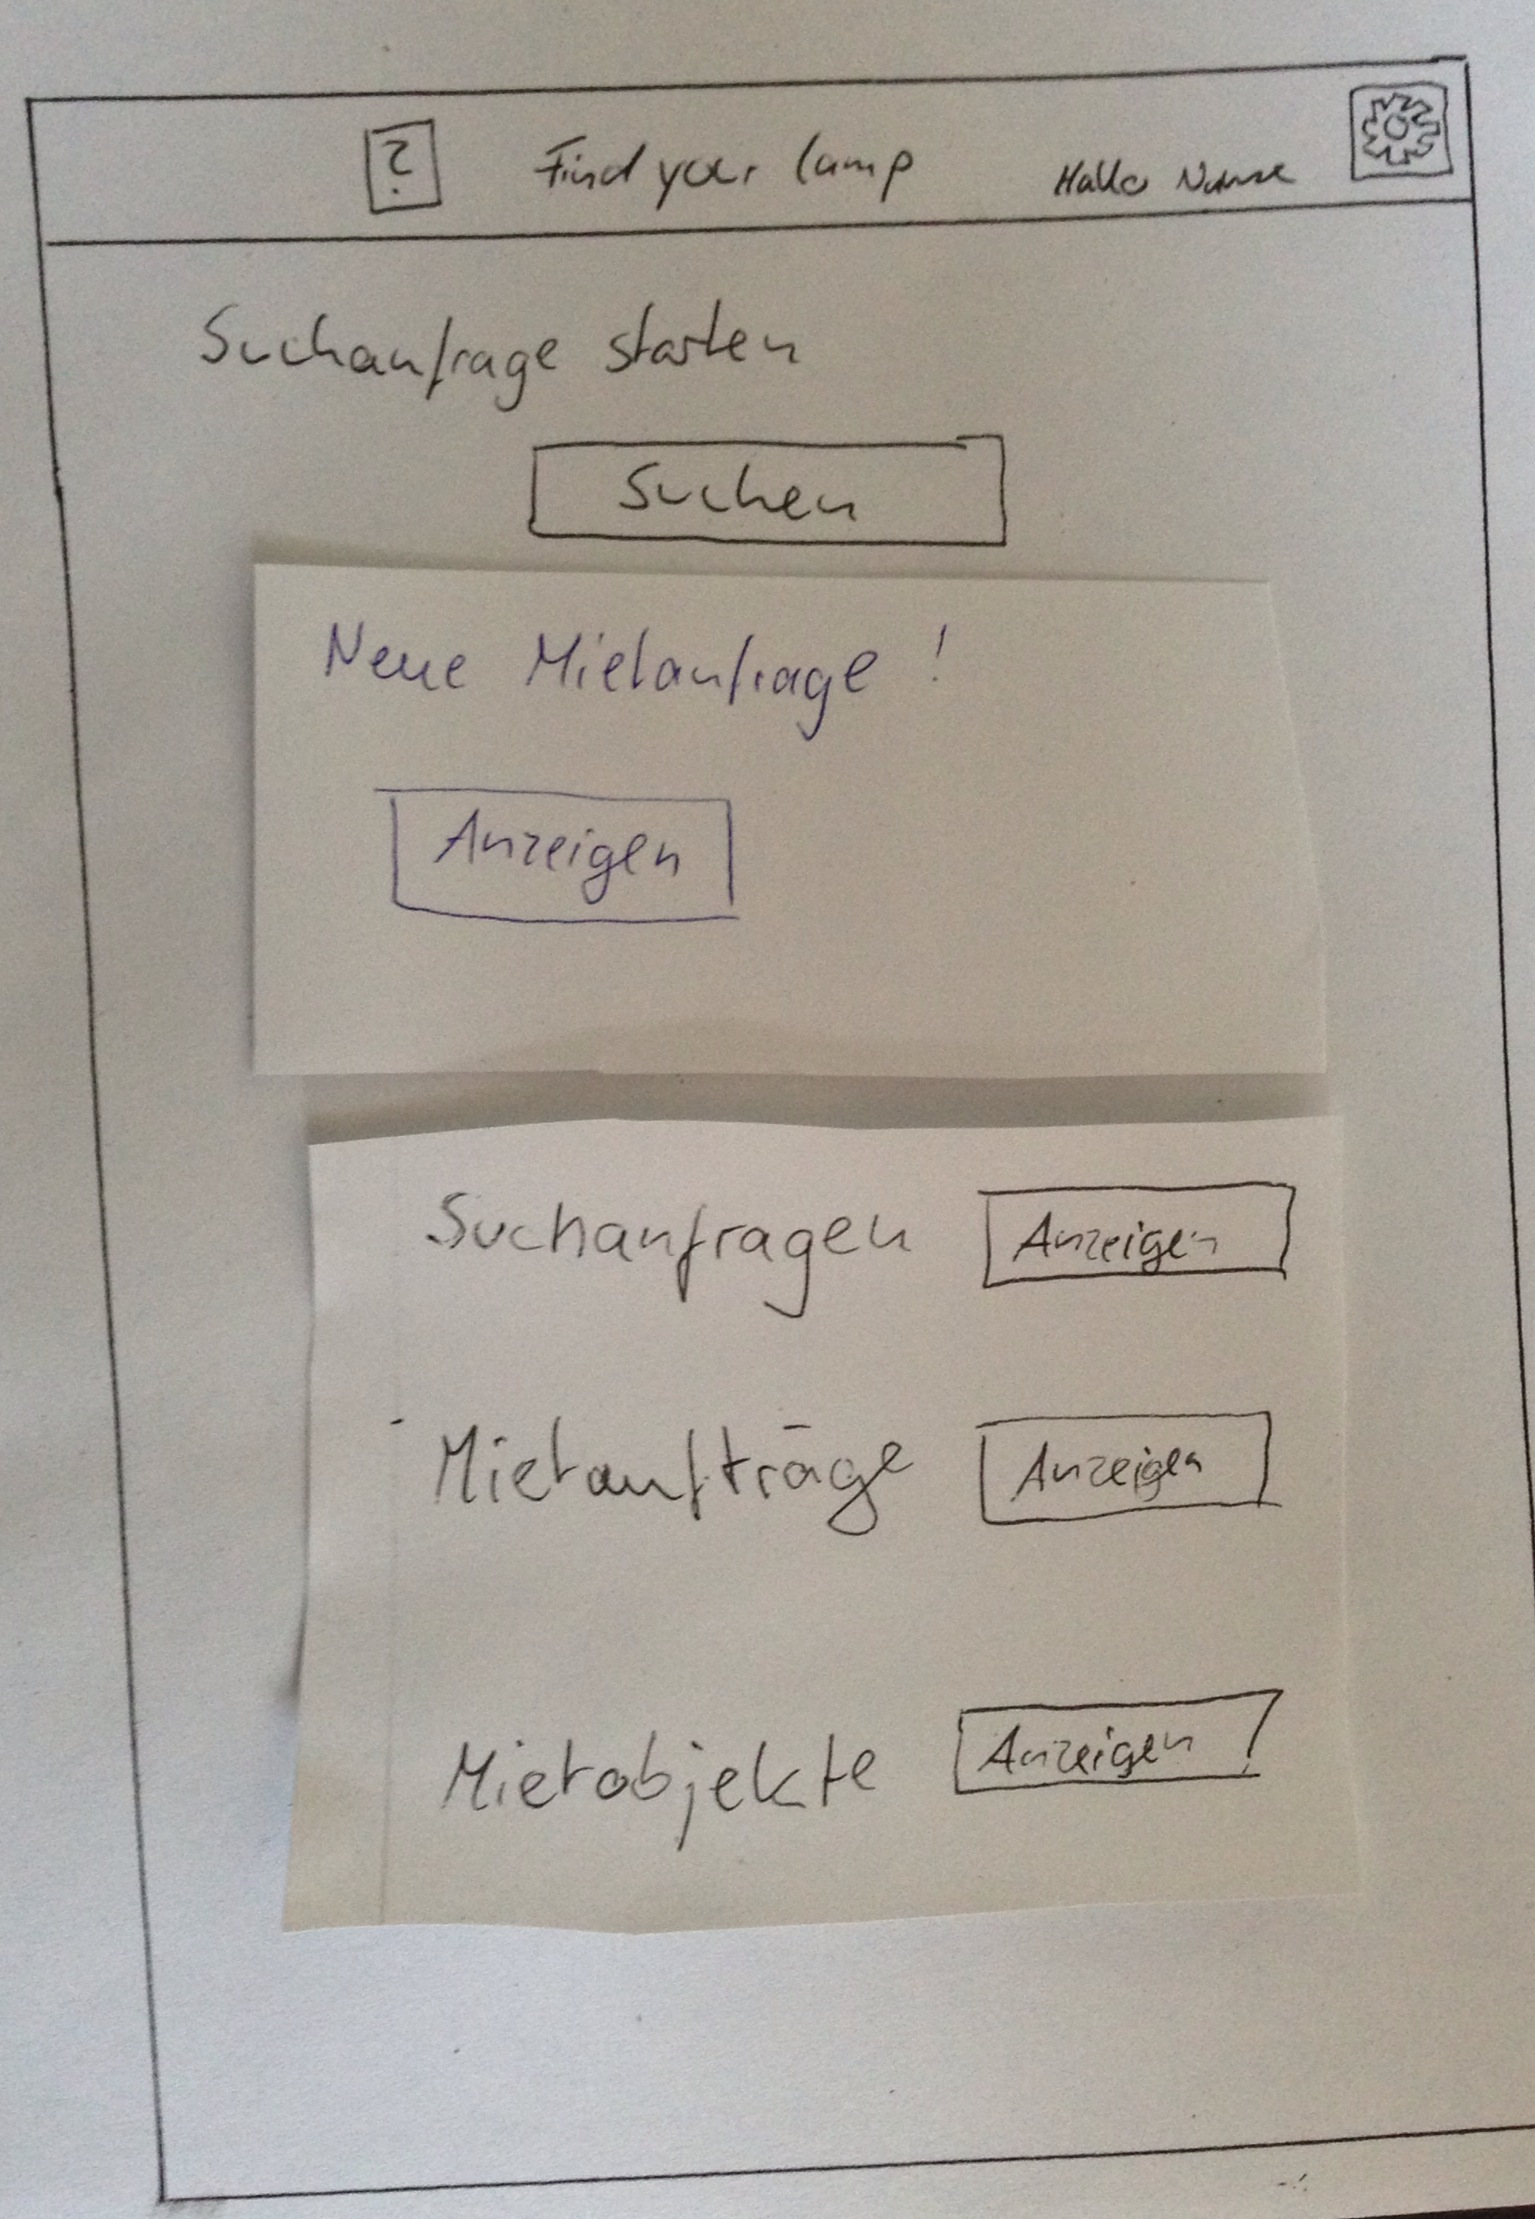
\includegraphics[angle=90, width=0.85\textwidth]{./images/paperbased/neueMietanfrage.JPG}
\caption{Pb Prototype: Mitteilung zur neuen Mietanfrage}
\label{pbprototype8}
\end{figure}

\begin{figure}[H]
\centering
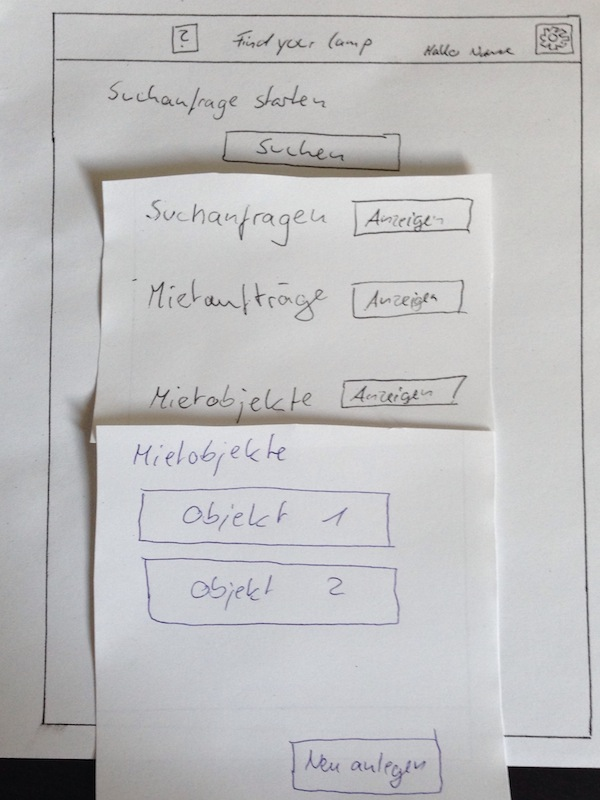
\includegraphics[angle=90, width=0.85\textwidth]{./images/paperbased/objekte.JPG}
\caption{Pb Prototype: Übersicht aller (eigenen) Mietobjekte}
\label{pbprototype9}
\end{figure}

\begin{figure}[H]
\centering
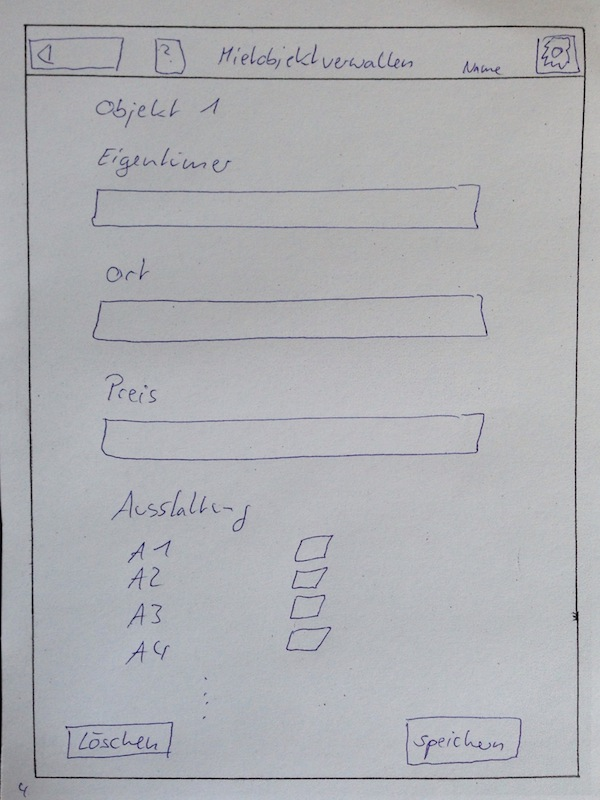
\includegraphics[angle=90, width=0.85\textwidth]{./images/paperbased/objektveralten.JPG}
\caption{Pb Prototype: Verwalten des Mietobjektes}
\label{pbprototype10}
\end{figure}

\begin{figure}[H]
\centering
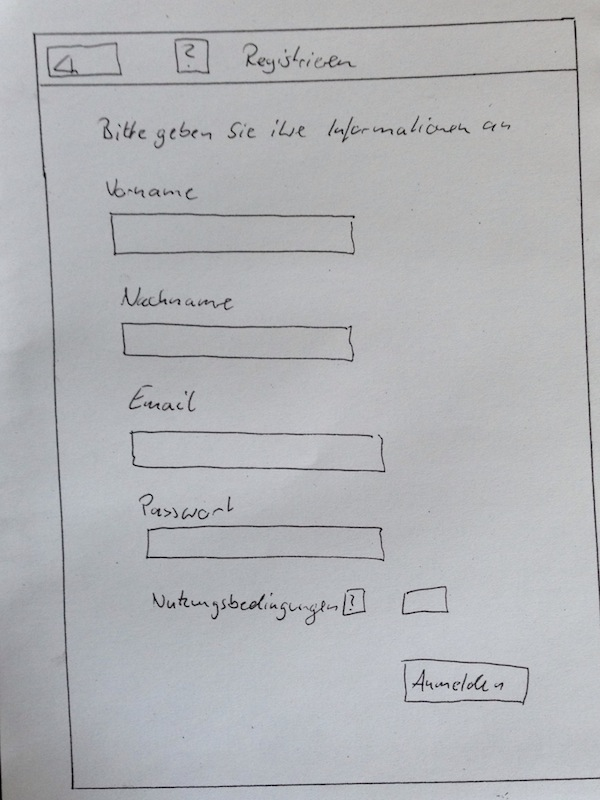
\includegraphics[angle=90, width=0.85\textwidth]{./images/paperbased/registrieren.JPG}
\caption{Pb Prototype: Registrierung}
\label{pbprototype11}
\end{figure}

\begin{figure}[H]
\centering
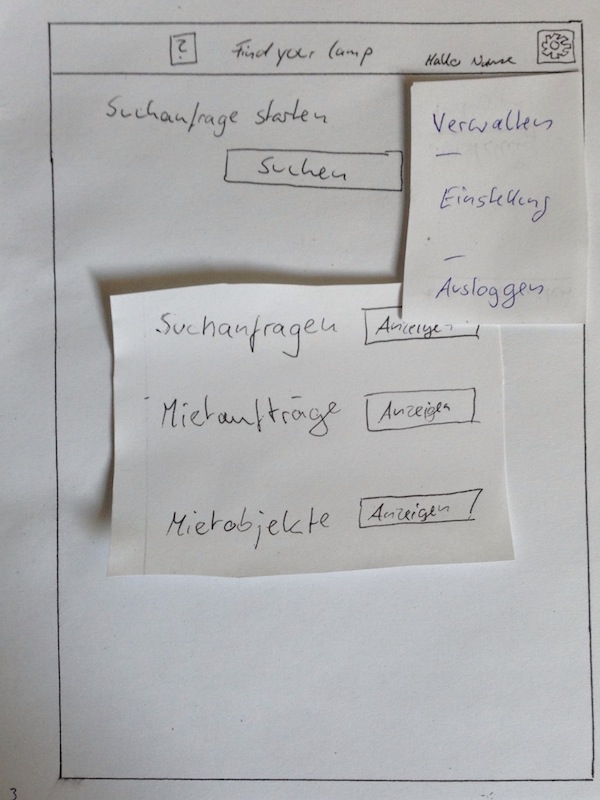
\includegraphics[angle=90, width=0.85\textwidth]{./images/paperbased/settings.JPG}
\caption{Pb Prototype: Einstellungen aktiv}
\label{pbprototype12}
\end{figure}

\begin{figure}[H]
\centering
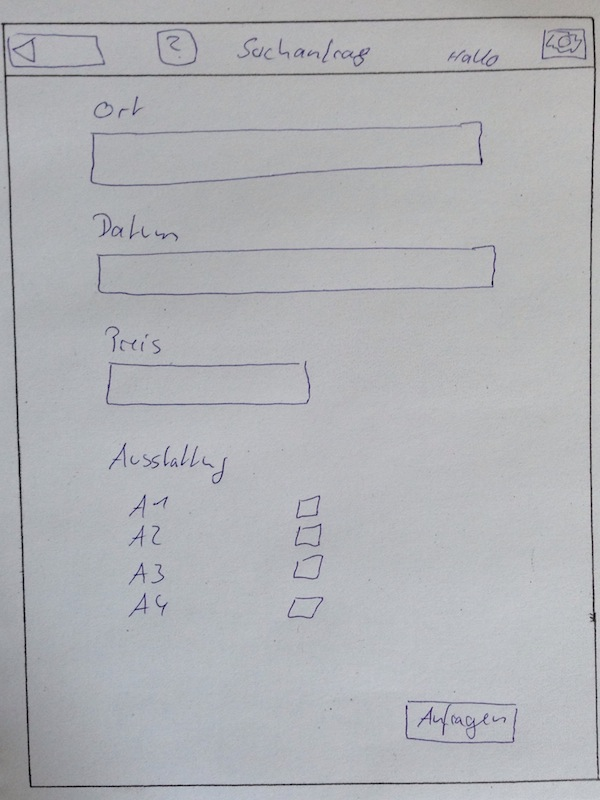
\includegraphics[angle=90, width=0.85\textwidth]{./images/paperbased/suchanfrage.JPG}
\caption{Pb Prototype: Starten einer neuen Suchanfrage}
\label{pbprototype13}
\end{figure}

\begin{figure}[H]
\centering
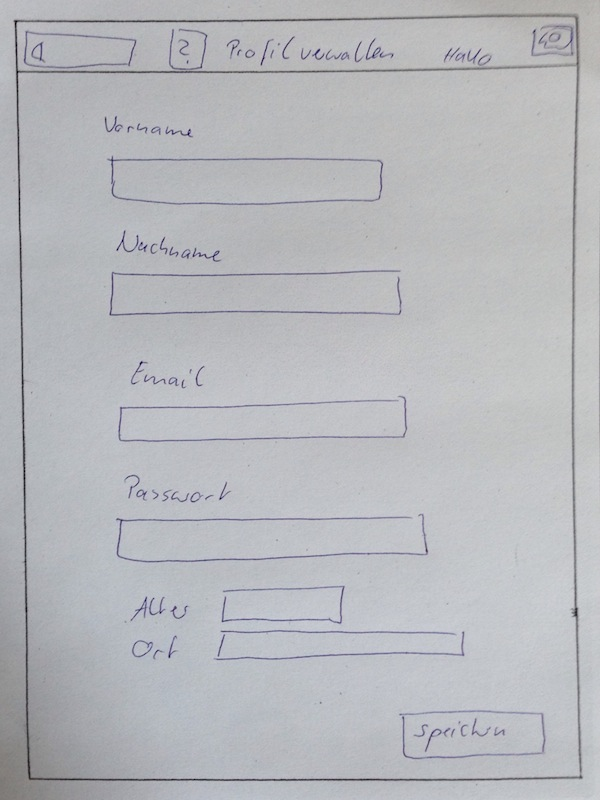
\includegraphics[angle=90, width=0.85\textwidth]{./images/paperbased/verwalten.JPG}
\caption{Pb Prototype: Verwalten des Benutzerprofils}
\label{pbprototype14}
\end{figure}

 \newpage
 %Konzeptpdf einbinden
\chapter{Konzept}
 Nachfolgend das überarbeitete Konzept.
 \includepdf[pages=1-, scale=1]{../konzept/konzept.pdf}


